\documentclass[10pt,journal,compsoc]{IEEEtran}

\usepackage{amsmath,amsfonts,amssymb,bm}
\usepackage{algorithmic}
\usepackage{algorithm}
\usepackage{array}
\usepackage{booktabs}
\usepackage[caption=false,font=footnotesize,labelfont=sf,textfont=sf]{subfig}
\usepackage{textcomp}
\usepackage{url}
\usepackage{verbatim}
\usepackage{graphicx}
\usepackage{multirow}
\usepackage[nocompress]{cite}
\hyphenation{op-tical net-works semi-conduc-tor}
\graphicspath{{../figures/}{../figures/scenes/}{../figures/paper/}}
\setlength{\textfloatsep}{6pt plus 1pt minus 2pt}
\setlength{\floatsep}{5pt plus 1pt minus 1pt}
\setlength{\intextsep}{6pt plus 1pt minus 2pt}
\setlength{\dbltextfloatsep}{6pt plus 1pt minus 2pt}
\setlength{\dblfloatsep}{5pt plus 1pt minus 1pt}
\setlength{\abovecaptionskip}{3pt}
\setlength{\belowcaptionskip}{0pt}
\makeatletter
\g@addto@macro\normalsize{%
  \setlength{\abovedisplayskip}{4pt plus 1pt minus 1pt}%
  \setlength{\belowdisplayskip}{4pt plus 1pt minus 1pt}%
  \setlength{\abovedisplayshortskip}{2pt plus 1pt minus 1pt}%
  \setlength{\belowdisplayshortskip}{3pt plus 1pt minus 1pt}%
}
\makeatother

\newcommand{\method}{\textsc{DOOR}}
\newcommand{\doorplus}{\textsc{DOOR+}}
\begin{document}
\raggedbottom

\title{Typed Budgets and Reliable Relations for Object-Relational Driving World Models}

\author{Peinan~Li,
        Zhiwen~Chen,
        Yibo~Song,
        Ruiyang~Gao,
        Yixiang~Yang,
        Ke~Wang,
        and~Zhipeng~Zhang$^{\ast}$%
\thanks{$^{\ast}$Corresponding Author.}%
\thanks{Peinan Li, Zhiwen Chen, Yibo Song, Ruiyang Gao, and Yixiang Yang are with AutoLab, SAI, Shanghai Jiao Tong University, Shanghai, China.}%
\thanks{Ke Wang is with Voyager Research, KargoBot, Beijing, China.}%
\thanks{Primary contact: zhipeng.zhang.cv@outlook.com; peinan\_li@163.com.}}

\markboth{IEEE Transactions on Pattern Analysis and Machine Intelligence}%
{Li \MakeLowercase{\textit{et al.}}: Typed Budgets and Reliable Relations for Driving World Models}

\IEEEtitleabstractindextext{%
% \begin{abstract}
% Object-relational world models expose interaction cues to a driving policy, but a fixed-capacity latent model still has to choose which tokens to keep. We cast that choice as budget allocation. \method\ selects dynamic-agent tokens and relation tokens under separate budgets before passing them to a shared world model. The design targets a simple failure mode: relation tokens added to the same top-$K$ pool as dynamic agents can push out the agents that the policy must track. Under a fair 16-slot budget on nuScenes, \method\ reduces rare-agent displacement error by 55.2\% and improves interaction recall at 1\,m by 8.3 points over object-only, while naive relation mixing degrades sharply. Policy behavior is less uniform. On nuScenes short-horizon latent imagination, object-only is the strongest Stage-1 baseline. On planning-oriented nuPlan, the no-visibility decoupled variant gives the strongest return at both 20k and 50k scale while lowering imagined collision rate relative to object-only. At 50k, it obtains $14.51 \pm 2.93$ return and $0.259 \pm 0.045$ collision rate, compared with $1.72 \pm 17.89$ and $0.610 \pm 0.146$ for object-only. A 50k offline planner-like evaluation also gives lower teacher-action MSE ($6.63 \pm 0.11$ versus $8.86 \pm 0.37$). Cross-dataset rollouts and nuScenes horizon sensitivity point to the same split: typed budgets improve the representation, but policy gains appear only when the evaluation can use relation tokens.
% \end{abstract}

\begin{abstract}
Object-relational world models expose interaction cues to autonomous-driving policies, but a bounded latent context must still decide which entities and relations survive compression. Existing shared top-$K$ selectors make dynamic-agent and relation tokens compete for the same slots, which can preserve high-risk relational warnings while discarding the agents needed to act on them. We formulate this as \emph{inter-type budget competition} and propose \method, a typed-budget abstraction that makes dynamic-agent and relation capacity explicit under a fixed total context. Our central finding is that capacity matters twice: it first determines representation sufficiency, and then constrains downstream imagination-policy utility. Stage-0 capacity scaling on nuScenes reveals distinct regimes. At $K=16$, shared object-relation selection is unstable (Dyn Rollout $38.41 \pm 27.90$, Rare ADE $7.15 \pm 4.79$, IntRec@1m $0.44 \pm 0.31$), while \method\ restores dynamic coverage and interaction recall (Dyn Rollout $0.73 \pm 1.05$, Rare ADE $0.44 \pm 0.15$, IntRec@1m $0.99 \pm 0.02$). At $K=32$, typed allocation gives the strongest compact representation trade-off, reaching IntRec@1m $1.00 \pm 0.00$ with low Dyn Rollout ($0.10 \pm 0.12$) and Rare ADE ($0.23 \pm 0.07$). At $K=64$, the gap narrows, showing that larger contexts can mitigate competition but at higher repeated-rollout memory and slot-interaction cost. A three-seed nuPlan Stage-1 K-scaling study further shows policy transfer for DOOR: return improves from $-11.96 \pm 7.67$ at $K=16$ to $1.17 \pm 3.36$ at $K=32$ and $14.88 \pm 0.78$ at $K=64$, while matched H=10 rollout memory rises from $110.9$ MB to $288.3$ MB. Finally, \doorplus\ is introduced as a separate reliability module: a trainable confidence-aware relation selector that suppresses false-positive high-risk relation slots without claiming universal policy improvement. These results support a broader principle: compact driving world models need both type-level capacity allocation for efficiency and reliability-aware relation control for perception-induced noise.
\end{abstract}


\begin{IEEEkeywords}
Autonomous driving, world models, object-relational representation, policy learning.
\end{IEEEkeywords}}

\maketitle
\IEEEdisplaynontitleabstractindextext

\section{Introduction}
\IEEEPARstart{W}{orld} models have emerged as a transformative paradigm for autonomous driving, enabling policies to train on imagined future trajectories rather than relying exclusively on costly, risk-sensitive, and sample-inefficient environmental interactions \cite{ha2018worldmodels,hafner2025dreamerv3}. However, driving is fundamentally a multi-agent interactive game governed by strict physical and topological constraints. To make safe and informed decisions, a driving policy cannot rely on an unstructured, flat latent embedding that entangles all scene elements. Instead, it must explicitly track a critical subset of dynamic agents (\textit{e.g.}, vehicles, pedestrians) alongside the relational structures (\textit{e.g.}, time-to-collision, lane conflicts, right-of-way) that dictate their interactions. 

This compositional requirement introduces a fundamental architectural challenge: \emph{how should relation-aware structures be integrated into a bounded-capacity latent driving model?} The issue is not that full-context modeling is impossible in principle. Rather, real-time driving world models usually communicate with planners and policies through a compact interface, such as learned queries, object slots, BEV cells, planner tokens, or a pruned entity set. Repeated imagination rollouts make this bottleneck especially important: increasing context size affects not only one encoder pass, but every recurrent dynamics step. A prevalent, albeit naive, approach is to append relation tokens to the same candidate pool as dynamic agents, operating under the assumption that an attention mechanism or a shared scoring network can optimally select the most critical tokens regardless of their semantic type.

In the context of autonomous driving, we identify this shared-bottleneck assumption as highly brittle. Relational features are inherently dependent on the entities they describe. A time-to-collision warning or a lane-conflict indicator provides actionable value to the policy only if the specific agents involved in that relation are simultaneously preserved within the latent state. When forced to compete in a single top-$K$ pool, high-risk relation tokens frequently crowd out the very dynamic agents they refer to. Consequently, the latent state may contain warnings about an impending interaction while missing the physical agent states needed to imagine the effect of an ego action.

We formalize this issue as an \emph{inter-type budget competition} problem within bounded-capacity abstraction. Given a candidate token set $\mathcal{V}_t$ and a total context budget $K$, the abstraction selects a subset $\mathcal{S}_t \subseteq \mathcal{V}_t$ with $|\mathcal{S}_t|\le K$ to maximize downstream utility $U(\mathcal{S}_t)$, including world-model prediction, interaction recall, and policy usefulness. The key question is therefore not whether a larger context can eventually recover more information, but which allocation policy gives the best decision-sufficient representation under a fixed compute interface. To address this, we propose \method, a typed-budget object-relational abstraction. \method\ strictly decouples the selection process, allocating separate token budgets for dynamic agents and relational interactions before feeding the aggregated slots to a shared reactive world model. Our core hypothesis is that typed budgeting preserves decision-critical dynamic coverage while retaining a reserved capacity for the highest-risk relational cues, all without expanding the total latent context size.

Beyond architectural design, this paper investigates a deeper scientific question: \emph{does an enhanced relational representation inherently translate to improved policy learning?} Better predictive metrics in a world model do not automatically simplify latent policy optimization. To rigorously decouple these effects, we design a two-stage evaluation protocol. Stage 0 measures representation sufficiency, specifically dynamic forecasting and rare-agent tracking, under controlled capacity scaling on nuScenes. Stage 1 then evaluates imagination-based policy learning across both the short-horizon nuScenes~\cite{caesar2020nuscenes} benchmark and the denser, planning-oriented nuPlan~\cite{caesar2021nuplan} benchmark at the 20k and 50k scales. We additionally run a clean Stage-1 DOOR K-scaling study to test whether representation capacity transfers to downstream imagination-policy utility.


Our comprehensive evaluation reveals a capacity-dependent relation between representation quality and downstream policy utility. In Stage 0, \method\ avoids the catastrophic failure mode of naive mixing, reducing rare-agent displacement error by 55.2\% and improving Interaction Recall@1m by 8.3 points under the compact reference setting. Capacity scaling shows that this is not an argument against larger contexts: $K=64$ reduces competition for all structured variants, but with substantially higher rollout memory and quadratic slot-interaction cost. Stage 1 then shows that capacity matters again for policy learning. On nuPlan, a clean DOOR K-scaling study improves return from $-11.96 \pm 7.67$ at $K=16$ to $1.17 \pm 3.36$ at $K=32$ and $14.88 \pm 0.78$ at $K=64$, with $K=32$ serving as a compact trade-off rather than a global optimum. The broader cross-dataset study remains nuanced: on nuScenes, object-only representations remain strongest, while on the complex nuPlan 50k benchmark the decoupled no-visibility variant outperforms object-only baselines, achieving a higher return ($14.51 \pm 2.93$ vs.\ $1.72 \pm 17.89$) and a lower imagined collision rate ($0.259 \pm 0.045$ vs.\ $0.610 \pm 0.146$). Offline planner-like evaluations and interaction-conditioned subset analyses further confirm that \method\ excels precisely in scenarios dominated by lane conflicts and low time-to-collision events.

The scope of this study is deliberately focused. Rather than presenting a monolithic perception-to-control system, we first study decision-sufficient abstraction using oracle tokens. This targeted protocol isolates the representation-policy interface and answers how latent capacity allocation affects downstream control. We then reintroduce controlled token perturbations as evaluation-time probes, showing which parts of the abstraction remain stable under localization noise, missing tokens, and false-positive high-risk relations.

% Figure~\ref{fig:teaser} illustrates the high-level conceptual motivation of our approach.

In summary, the main contributions of this work are:
\begin{enumerate}
\item We define \emph{inter-type budget competition} in bounded-capacity object-relation driving world models, showing that naively mixing relation tokens into a shared bottleneck degrades dynamic-agent coverage and can harm downstream policy learning.
\item We propose \method, a typed-capacity abstraction that separates dynamic-agent and relation-token budgets under the same total slot count, making the allocation policy explicit and diagnosable rather than hidden inside a shared top-$K$ selector.
\item We provide capacity-scaling and split-sweep evidence showing that typed allocation improves compact-budget Pareto efficiency: it is most valuable at compact and medium budgets, while larger contexts reduce competition at higher rollout memory and slot-interaction cost, and the best type split depends on dataset statistics and metric emphasis.
\item We show that capacity matters beyond representation. A clean three-seed Stage-1 DOOR K-scaling study on nuPlan demonstrates that downstream imagination return improves from $K=16$ to $K=32$ and $K=64$, connecting representation sufficiency to policy utility while preserving the compute trade-off.
\item We diagnose relation utility and reliability. Long-horizon interventions show that, in the current nuPlan setting, TTC/risk dominates the effective relation channel, while perception-noise stress tests identify false-positive high-risk relations as the main remaining failure mode.
\item We introduce \doorplus, a trainable confidence-token relation selector that mitigates relation-slot contamination from false positives. Under H=10/20/50 rollouts, \doorplus\ keeps selected false-positive relation occupancy near zero while maintaining clean-level return and only minor collision degradation under relfp0.2. Confidence ablations show a causal gradient from normal, to shuffled/constant, to inverted confidence. We evaluate \doorplus\ as a relation-reliability mechanism, not as a universal Stage-1 policy optimizer.
\end{enumerate}



% \IEEEPARstart{W}{orld} models have emerged as a powerful paradigm for autonomous driving, enabling policies to train on imagined trajectories rather than relying exclusively on expensive and risk-sensitive environmental interactions \cite{ha2018worldmodels,hafner2025dreamerv3}. However, standard monolithic latent states struggle to capture the compositional and highly interactive nature of driving scenes. To make informed decisions, a driving policy cannot rely on a shapeless global vector. Instead, it must explicitly track a critical subset of dynamic agents alongside the relational structures that dictate their interactions. 

% This requirement introduces a fundamental architectural challenge regarding how relation-aware structures should be integrated into a fixed-capacity latent driving model. A prevalent approach is to append relation tokens to the same top-$K$ bottleneck used for dynamic agents, operating under the assumption that all token types should compete for the same representational slots. In the context of autonomous driving, this naive mixing strategy proves highly brittle. Relational features, such as lane-conflict indicators or time-to-collision estimates, are inherently dependent on the entities they describe. They provide actionable value only if the agents involved in that specific relation are simultaneously preserved within the latent state. 

% We identify this bottleneck issue fundamentally as a budget-allocation problem. The efficacy of relation-aware driving world models depends entirely on how representational slots are distributed across heterogeneous token types. To address this, we propose \method\, a novel architecture that selects dynamic-agent tokens and relation tokens under strictly separate budgets before feeding the aggregated slots to a shared world model. Our core hypothesis is that naive relation mixing forces relation tokens to compete directly with dynamic agents, inadvertently discarding the very entities required for downstream control.

% Beyond representation design, a critical open question is whether enhanced relational forecasting inherently translates to improved policy learning. Better predictive metrics do not automatically simplify latent policy optimization. To investigate this, we conduct a comprehensive two-stage evaluation. We first assess representation quality under a fair 16-slot budget on the nuScenes dataset, followed by an evaluation of imagination-based policy learning across both nuScenes and the planning-oriented nuPlan benchmark. 

% Our findings reveal a nuanced relationship between representation and policy performance. While decoupled typed-budget representations consistently demonstrate superior forecasting capabilities across datasets, the downstream policy benefits are highly context-dependent. On nuScenes, where relational cues are less critical for the specific evaluation metrics, object-only representations remain highly competitive. However, on the more complex nuPlan benchmark at both 20k and 50k scales, the ranking dramatically flips. Our decoupled architecture achieves the strongest returns and significantly improves collision avoidance compared to object-only baselines. Offline planner-like evaluations, cross-dataset transfer experiments, and horizon sweeps further corroborate this trend. Ultimately, we demonstrate that while typed budgets universally improve state abstraction, policy gains materialize primarily when the evaluation environment possesses sufficient complexity to exploit relational tokens.

% Rather than presenting a monolithic perception-to-control system, our study focuses specifically on decision-sufficient abstraction for imagination-based policy learning. This targeted approach allows us to rigorously isolate and analyze the representation-policy interface without the confounding variables typical of large closed-loop benchmarks. 

% Figure~\ref{fig:teaser} illustrates the high-level architecture and conceptual motivation of our approach.

% The main contributions of this work are summarized as follows:
% \begin{enumerate}
% \item We identify and formalize \emph{inter-type budget competition} in relation-aware latent driving models, demonstrating that naively mixing relation tokens into a shared bottleneck severely degrades dynamic-agent coverage under fixed latent budgets.
% \item We propose \method\, a typed-budget object-relational abstraction that explicitly decouples dynamic-agent and relation-token selection while maintaining a constant total world-model context size.
% \item We provide a comprehensive evaluation revealing a fundamental decoupling between representation sufficiency and policy utilization. We show that while typed budgeting consistently improves latent representations, significant policy gains depend heavily on the relational complexity of the downstream task.
% \end{enumerate}



% \IEEEPARstart{W}{orld} models let driving policies train on imagined trajectories instead of direct environment interaction \cite{ha2018worldmodels,hafner2025dreamerv3}. That is attractive in driving, where trial-and-error is expensive and risk-sensitive. The state representation cannot be a shapeless global vector: the policy must track a few agents and the relations that make them relevant.

% This leads to a concrete representation question: \emph{how should relation-aware structure enter a fixed-capacity latent driving model?} A common answer is to append relation tokens to the same top-$K$ bottleneck used for dynamic agents. That assumes all token types should compete for the same slots. In driving, this is brittle. A lane-conflict or time-to-collision token only helps if the agents involved in that relation are still present in the latent state.

% The issue is a budget-allocation problem. Relation-aware driving world models depend on what they encode and on how slots are divided across token types. \method\ selects dynamic-agent tokens and relation tokens under separate budgets, then feeds the selected slots to a shared world model. The hypothesis is narrow: naive relation mixing makes relation tokens compete with dynamic agents and can remove the entities needed for control.

% The next question is whether the representation gain helps policy learning. Better forecasting metrics need not make latent policy optimization easier. Stage 0 measures representation quality under a fair 16-slot budget on nuScenes. Stage 1 evaluates imagination-based policy learning on nuScenes and on a planning-oriented nuPlan benchmark.

% There is no single global ranking. On nuScenes, Stage 0 favors the decoupled typed-budget representation, but Stage 1 still favors object-only. On nuPlan 20k and 50k, the ranking flips: the decoupled no-visibility variant gives the strongest return while improving collision behavior over object-only, and an offline planner-like evaluation gives the same ordering. Cross-dataset transfer and horizon sweeps lead to the same reading. Typed budgets improve the representation; policy gains depend on the dataset and token statistics.

% The scope is deliberately limited. The paper studies decision-sufficient abstraction for imagination-based policy learning, not a full perception-to-control system or a large closed-loop benchmark. This keeps the representation-policy interface visible.

% Figure~\ref{fig:teaser} gives the high-level picture.

% The contributions are:
% \begin{enumerate}
% \item An account of \emph{inter-type budget competition} in relation-aware latent driving models: naively mixing relation tokens into a shared bottleneck can degrade dynamic-agent coverage under a fixed latent budget.
% \item \method, a typed-budget object-relational abstraction that decouples dynamic-agent and relation-token selection while keeping the total world-model context fixed.
% \item A two-stage evaluation showing that typed budgeting improves representation sufficiency on nuScenes, while policy gains remain dataset-dependent: object-only leads on nuScenes Stage 1, and the no-visibility decoupled variant leads the nuPlan return metric, offline planner-like evaluation, and transfer checks.
% \end{enumerate}

\begin{figure*}[!t]
\centering
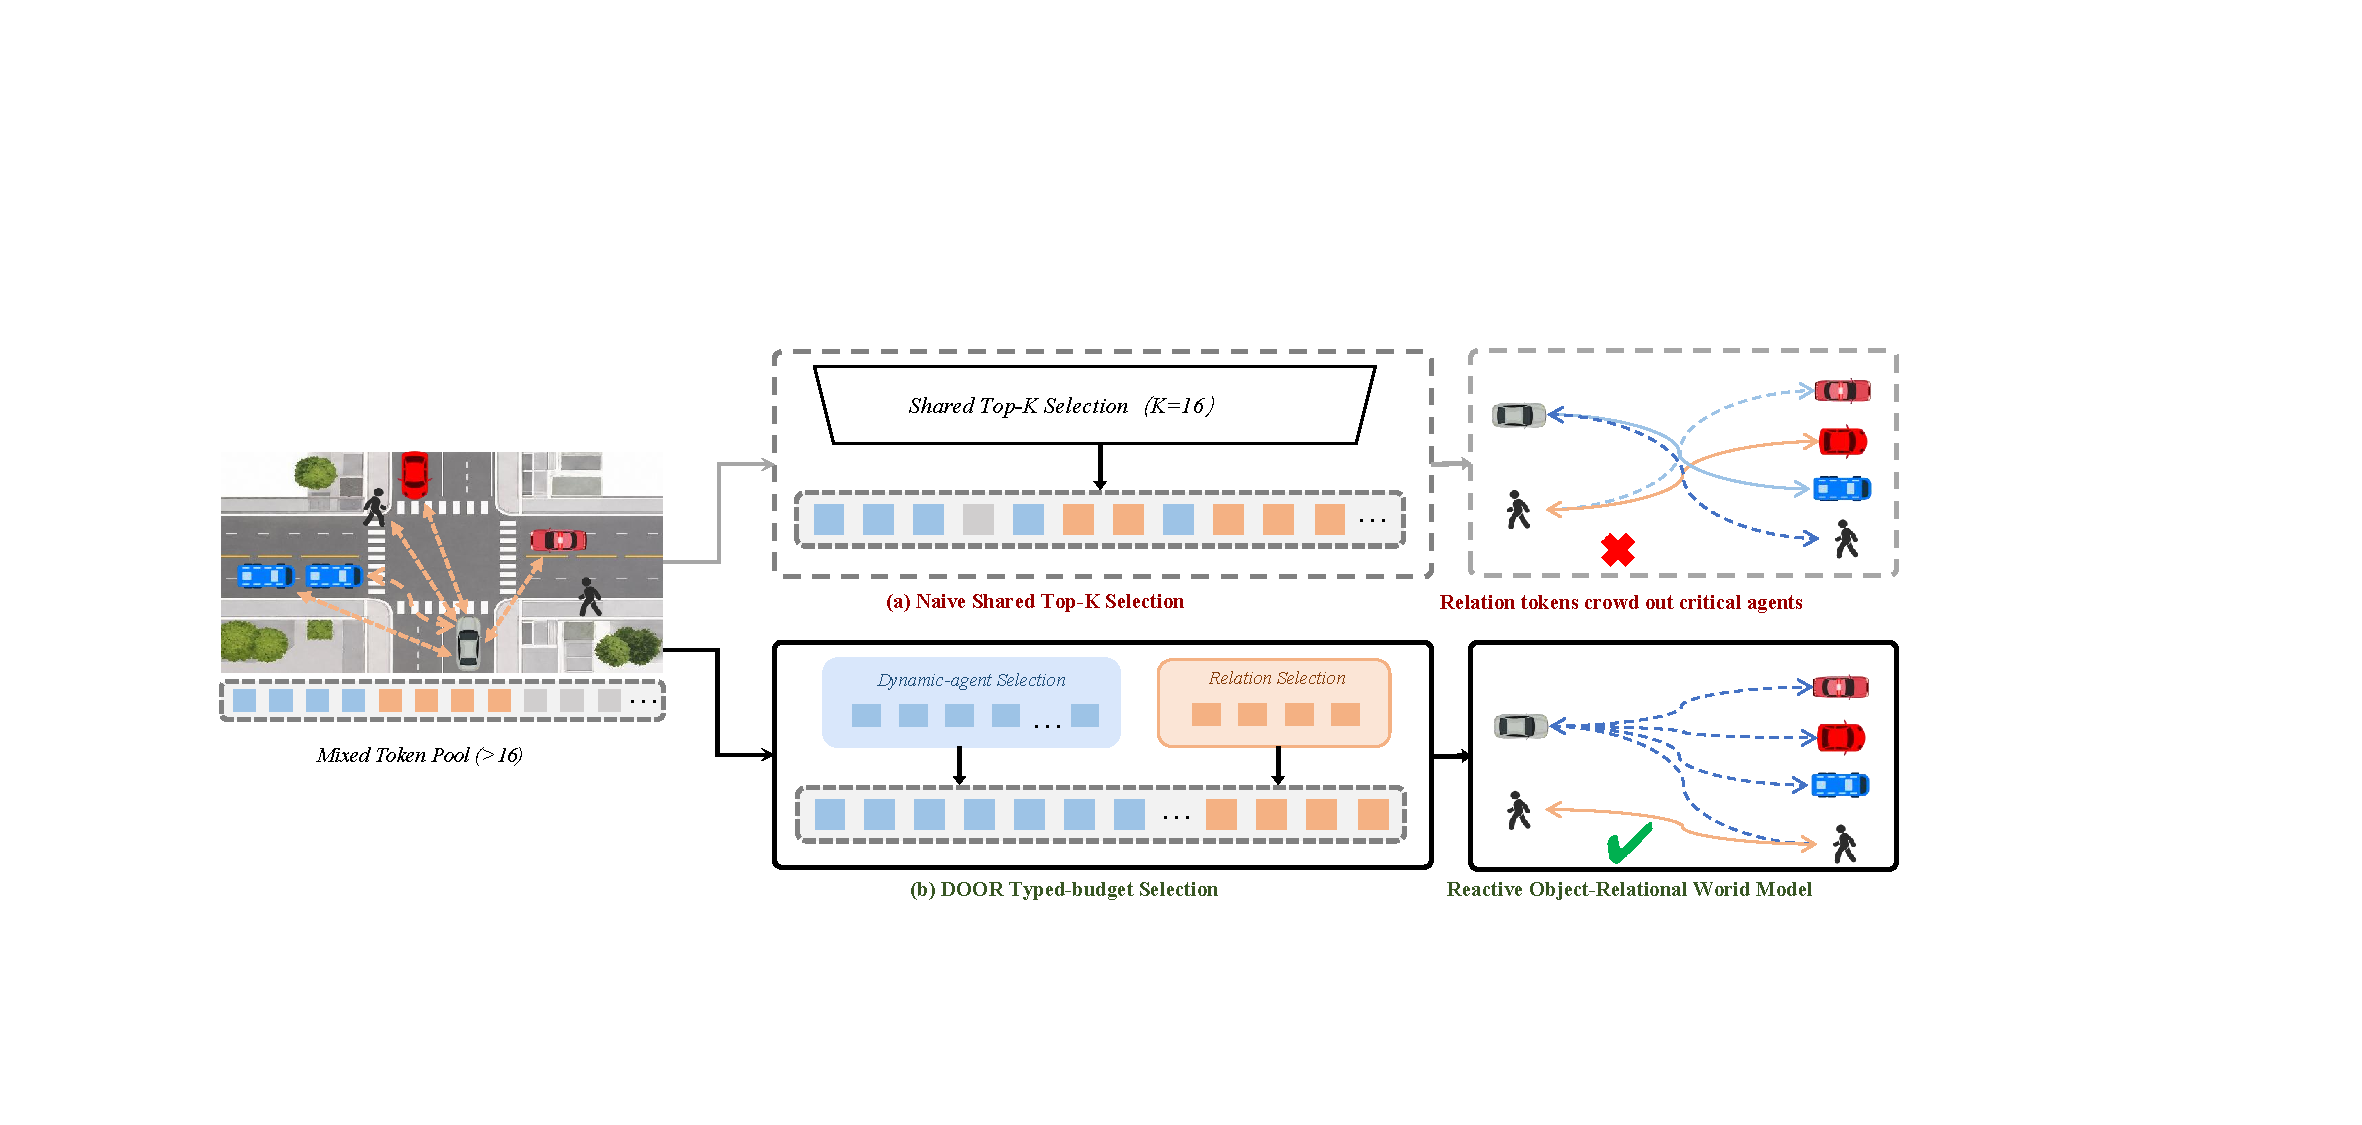
\includegraphics[width=\textwidth]{../figures/fig1.pdf}
\caption{Overview. Under a bounded latent budget, naive shared object-relation selection can displace decision-critical dynamic agents. Typed-budget decoupling restores that context in compact regimes; increasing capacity further improves downstream policy utility at higher repeated-rollout cost. \doorplus\ separately improves reliability of the reserved relation slots under false-positive relation noise.}
\label{fig:teaser}
\end{figure*}



\section{Related Work}
\subsection{World Models for Driving Policy Learning}
World models train policies through learned latent rollouts rather than direct environment interaction \cite{ha2018worldmodels,hafner2019planet,hafner2020dreamer,hafner2021mastering,hafner2025dreamerv3}. The idea is rooted in model-based reinforcement learning and planning-through-simulation, from Dyna-style updates to modern latent planners and model-based policy optimization \cite{sutton1991dyna,janner2019mbpo,kaiser2020modelbased,schrittwieser2020muzero,hansen2022tdmpc}. Driving makes this appealing because online trial-and-error is costly and risk-sensitive. Model-based driving systems and imitation frameworks use learned dynamics, compact scene states, or planner-like supervision to reduce online interaction \cite{chen2021worldonrails,hu2022mile,bansal2019chauffeurnet,codevilla2018conditional}. These works usually keep the latent scene interface fixed. Here the interface itself is under study: we ask whether the world model is given a decision-sufficient set of entities and relations before any policy update occurs.

\subsection{Object-Centric and Relational Representations}
Object-centric learning represents scenes using discrete slots or entities \cite{greff2019multiobject,locatello2020slotattention}. Furthermore, relational inductive biases and graph reasoning explicitly model interactions, rather than relying on implicit inference from pooled embeddings \cite{santoro2017relation,battaglia2018relational,kipf2018nri}. Autonomous driving policies inherently require similar structural priors. Ego actions are continuously shaped by physical entities such as nearby vehicles and vulnerable road users, alongside relational factors including map constraints, right-of-way, lane conflicts, and time-to-collision. Earlier multi-agent prediction models already showed the value of interaction-aware futures and social context \cite{gupta2018socialgan,ivanovic2019trajectron,rhinehart2019precog,salzmann2020trajectronpp}. To expose these interactions and map structures, forecasting systems such as VectorNet, LaneGCN, TNT, DenseTNT, HiVT, and MultiPath++ employ vectorized agents, lane graphs, discrete goals, and multimodal futures \cite{gao2020vectornet,liang2020lanegcn,zhao2021tnt,gu2021densetnt,zhou2022hivt,varadarajan2022multipathpp}. Recent attention-based predictors further scale this paradigm using agent-map transformers, query-centric decoding, and compact attention patterns \cite{yuan2021agentformer,ngiam2022scene,shi2022mtr,nayakanti2023wayformer,zhou2023qcnet}. In contrast to these architectural advancements, our work addresses a more specific bottleneck. We investigate how pre-extracted object and relation tokens should be integrated into a fixed-capacity world model.

% Employing a naive shared top-$K$ bottleneck often retains an excess of relation tokens at the expense of the very agents those relations describe. Therefore, rather than merely validating the general utility of relational features, we examine whether such relational evidence remains physically grounded and actionable after undergoing severe latent compression.


% Object-centric learning represents scenes with slots or entities \cite{greff2019multiobject,locatello2020slotattention}. Relational inductive biases and graph reasoning make interactions explicit instead of leaving them to be inferred from a pooled embedding \cite{santoro2017relation,battaglia2018relational,kipf2018nri}. Driving policies need the same structure: nearby vehicles, vulnerable road users, map constraints, right-of-way, lane conflict, time-to-collision, and priority all affect the ego action. Forecasting systems such as VectorNet, LaneGCN, TNT, DenseTNT, and MultiPath++ use vectorized agents, lane graphs, discrete goals, and multimodal futures to expose interaction and map structure \cite{gao2020vectornet,liang2020lanegcn,zhao2021tnt,gu2021densetnt,varadarajan2022multipathpp}. Recent attention-based predictors further scale this idea with agent-map transformers, query-centric decoding, or compact attention patterns \cite{yuan2021agentformer,ngiam2022scene,shi2022mtr,nayakanti2023wayformer,zhou2023qcnet}. The question here is narrower: after object and relation tokens exist, how should they enter a fixed-capacity world model? A shared top-$K$ bottleneck can keep more relation tokens while losing the agents those relations refer to. This is different from asking whether relations are useful in principle; it asks whether relation evidence remains actionable after compression.

\subsection{Planning-Oriented Autonomous Driving}
Planning-oriented driving systems organize perception, prediction, and planning around structured scenes \cite{hu2022stp3,hu2023uniad,jiang2023vad}. These architectures build upon foundational methods that utilize rasterized, vectorized, occupancy-centric, or fused sensor encodings to generate ego trajectories subject to map and actor constraints \cite{zeng2019end,casas2021mp3,philion2020lift,transfuser2021,sadat2020perceive}. Object-level planners explicitly address this design pressure by providing the planner with direct access to agent states and route contexts \cite{renz2022plant}. While full end-to-end evaluations are comprehensive, they inherently conflate perception errors, supervision signals, simulator dynamics, and planning capabilities. To circumvent these confounding factors, our study utilizes oracle tokens to isolate a specific component of the autonomy stack. This targeted approach enables us to rigorously evaluate whether a typed allocation of dynamic-agent and relation-token capacity enhances latent world-model learning and successfully transfers to downstream policy optimization.


% Planning-oriented driving systems organize perception, prediction, and planning around structured scenes \cite{hu2022stp3,hu2023uniad,jiang2023vad}. They build on methods that use rasterized, vectorized, occupancy-centric, or fused sensor encodings to produce ego trajectories under map and actor constraints \cite{casas2021mp3,philion2020lift,transfuser2021,sadat2020perceive}. Object-level planners make the same design pressure explicit by exposing agents and route context directly to the planner \cite{renz2022plant}. Full end-to-end evaluation mixes perception, supervision, simulator behavior, and planning. Oracle tokens isolate one part of that stack: whether typed allocation of dynamic-agent and relation-token capacity improves latent world-model learning and transfers to policy optimization.

\subsection{Driving Benchmarks and Cross-Dataset Evaluation}
nuScenes \cite{caesar2020nuscenes}, Argoverse \cite{chang2019argoverse,wilson2023argoverse2}, Waymo Open Motion \cite{sun2020scalability,ettinger2021large}, and nuPlan \cite{caesar2021nuplan} stress different parts of the driving stack. CARLA \cite{dosovitskiy2017carla}, Waymax \cite{mao2023waymax}, and NAVSIM \cite{dauner2024navsim} make a related point from the simulator side: the downstream task changes the meaning of a representation. A representation that improves prediction on one dataset may not improve policy learning on another, especially when token statistics, visibility fields, teacher-action scales, and interaction density differ. We use this contrast by evaluating the same abstraction family on nuScenes short-horizon imagination and nuPlan planning-oriented imagination.

\section{Problem Formulation}
We consider a driving agent acting in a partially observable traffic environment. At time step $t$, the agent receives a structured scene representation
\begin{equation}
\mathbf{x}_t = \{\mathbf{e}_t, \mathcal{O}_t, \mathcal{M}_t, \mathcal{R}_t\},
\label{eq:state}
\end{equation}
where $\mathbf{e}_t$ denotes the ego token, $\mathcal{O}_t$ denotes dynamic-agent tokens, $\mathcal{M}_t$ denotes map tokens, and $\mathcal{R}_t$ denotes relation tokens. The policy $\pi(\mathbf{a}_t \mid \mathbf{x}_t)$ outputs a driving action $\mathbf{a}_t$, which may correspond to low-level control or a compact motion command.

The world model may receive many candidate scene tokens, but the planner-facing interface is bounded by a compact context budget $K$. We write the abstraction problem as
\begin{equation}
\mathcal{S}^{\star}_t
= \arg\max_{\mathcal{S}_t \subseteq \mathcal{V}_t,\ |\mathcal{S}_t|\le K}
U(\mathcal{S}_t),
\label{eq:bounded_abstraction}
\end{equation}
where $\mathcal{V}_t=\{\mathbf{e}_t,\mathcal{O}_t,\mathcal{M}_t,\mathcal{R}_t\}$ is the candidate token set and $U$ denotes decision utility induced by prediction accuracy, interaction preservation, and downstream policy behavior. Consequently, the fundamental challenge lies not only in \emph{what} to encode, but also in \emph{how} to allocate this limited capacity between dynamic-agent and relational information. If relation tokens compete within the same bottleneck as dynamic-agent tokens, they risk displacing the very entities crucial for control. To address this, the abstraction $A_\theta$ and the world model $f_\theta$ are trained to ensure that the latent state remains decision-sufficient for two distinct objectives: (1) \textbf{representation sufficiency}, which preserves dynamic prediction, rare-agent tracking, and interaction-critical structures under a fair bounded budget; and (2) \textbf{policy learning}, which enables stable, imagination-based policy optimization.

\paragraph{Why fixed capacity?}
The fixed-capacity assumption is not an arbitrary handicap. Modern driving world models and planners almost always communicate through a compressed interface: learned queries, object slots, BEV cells, planner tokens, or a bounded set of scene entities. This compression is required by latency, memory bandwidth, transformer attention cost, and the need to pass a stable context into recurrent imagination or policy heads. Our claim is therefore conditional but practically relevant: \emph{given a compact world-model context, how should heterogeneous scene information share that context?} We keep $K$ fixed within each comparison so that experiments compare allocation policies rather than raw model capacity, and then explicitly sweep $K$ to characterize the resulting regimes. The 97-token reference reported later is intentionally treated as a non-fair upper bound; it shows the headroom available when the bottleneck is mostly removed, not a deployable alternative under the same compute interface. Thus the contribution is not that $K=16$ is universal, nor that $K=32$ is globally optimal, but that typed capacity allocation improves the efficiency of compressed object-relation interfaces when increasing $K$ is constrained by repeated rollout cost.



% The world model cannot consume the full scene. It compresses $\mathbf{x}_t$ into a latent context of fixed capacity $K$. The problem is not only \emph{what} to encode, but also \emph{how} to allocate capacity between dynamic-agent and relation information. If relation tokens enter the same bottleneck as dynamic-agent tokens, they may displace the entities needed for control. The abstraction $A_\theta$ and world model $f_\theta$ are trained so that the latent state remains decision-sufficient for two tasks:
% \begin{enumerate}
% \item \textbf{Representation sufficiency:} preserve dynamic prediction, rare-agent tracking, and interaction-critical structure under a fair fixed latent budget.
% \item \textbf{Policy learning:} enable stable imagination-based policy optimization.
% \end{enumerate}

\subsection{Scope and Evaluation Assumptions}
The experiments study decision learning with structured scene tokens rather than full perception. In \emph{oracle-token evaluation}, scene tokens come from annotations, simulator state, or an equivalent trusted front-end. This removes perception noise from the abstraction-and-policy question. 

% The evidence concerns latent representation and imagination-based policy learning, not complete perception-to-control autonomy.

We use two criteria for a decision-sufficient abstraction. First, the selected context should preserve entities that the policy may need to react to, especially near-field dynamic agents and rare vulnerable road users. Second, it should preserve compact interaction evidence, such as low time-to-collision or lane conflict, without letting those relation tokens remove the entities that make the relation meaningful. A representation can satisfy one criterion and fail the other. Object-only selection keeps dynamic agents but lacks explicit interaction semantics; naive object-relation selection keeps relation tokens but can lose dynamic coverage. Typed budgets are designed to make this trade-off explicit.

\section{Method}
\subsection{Scene Tokenization}
Each scene is represented in an ego-centric local frame to encourage cross-benchmark consistency. The raw feature layout used by the current implementation contains a fixed-length token vector of dimension $D_{\mathrm{raw}}=40$, with the first coordinates reserved for relative position, velocity, object extent, risk proxies, visibility, time-to-collision, lane conflict, interaction priority, distance, heading, and token type. The maximum token budget is $S=97$, corresponding to one ego token, a bounded set of dynamic-agent tokens, map tokens, relation tokens, and padding.

% The design keeps the model interface stable across datasets and keeps relation features explicit. Relation tokens encode relative geometry, relative velocity, time-to-collision proxy, lane conflict, visibility, and interaction priority. The schema is shared across the two main Stage-1 settings, but the token statistics differ: nuScenes contains visibility variation, whereas the nuPlan preprocessed pipeline yields nearly constant visibility. This difference affects the visibility ablations.

The design keeps the interface stable across datasets and relation features explicit. Relation tokens encode relative geometry, relative velocity, time-to-collision proxy, lane conflict, visibility, and interaction priority. Both Stage-1 settings share this schema, yet token statistics differ since nuScenes contains visibility variation while nuPlan yields nearly constant visibility. This impacts visibility ablations.



% Table~\ref{tab:token_schema} summarizes the feature fields used by the implementation. Only the first 15 dimensions are semantically assigned; the remaining dimensions are reserved so that additional map, signal, or dataset-specific attributes can be added without changing the model interface. The ego token is always placed at slot 0. Dynamic-agent tokens are appended next, followed by map-anchor tokens, relation tokens, and padding. The nuPlan preprocessed adapter uses route-lane anchors before other lane anchors for map tokens, whereas the nuScenes adapter uses available local map information when present. Relation tokens are ego-object edges: for every dynamic object we compute relative displacement, relative velocity, time-to-collision, inverse-distance risk, a lane-conflict indicator, visibility, and priority. If more relation edges are available than the relation-token cap, they are sorted by risk and the highest-risk edges are retained.

\begin{table}[!t]
\caption{Raw token fields used by the structured scene interface.}
\label{tab:token_schema}
\centering
\resizebox{\columnwidth}{!}{%
\begin{tabular}{lll}
\toprule
Dim. & Field & Notes \\
\midrule
0--1 & $(x,y)$ & ego-centric relative position \\
2--3 & $(v_x,v_y)$ & relative or local-frame velocity \\
4--5 & length, width & object extent when available \\
6 & risk & inverse-distance or adapter risk proxy \\
7 & visibility & nuScenes bin midpoint; nuPlan is 1.0 \\
8 & TTC & relation-token time-to-collision proxy \\
9 & lane conflict & 1 if lateral offset is below 2 m \\
10 & priority & interaction-priority heuristic \\
11 & distance & ego-object distance \\
12 & heading & local heading \\
13 & interactive flag & reserved interaction marker \\
14 & token type & ego/object/map/relation/pad id \\
15 & relation confidence & optional field used by \doorplus \\
16 & relation uncertainty & optional field used by \doorplus \\
\bottomrule
\end{tabular}}
\end{table}

Table~\ref{tab:token_schema} summarizes the feature fields used by the implementation. The first 17 dimensions are semantically assigned after adding \doorplus\ confidence fields; the remaining dimensions are reserved so that additional map, signal, or dataset-specific attributes can be added without changing the model interface. The ego token always occupies slot 0. Dynamic-agent tokens are appended next, followed by map-anchor tokens, relation tokens, and padding. The nuPlan preprocessed adapter uses route-lane anchors before other lane anchors for map tokens, whereas the nuScenes adapter uses available local map information. Relation tokens are ego-object edges: for every dynamic object we compute relative displacement, relative velocity, time-to-collision, inverse-distance risk, a lane-conflict indicator, visibility, and priority. If more relation edges are available than the relation-token cap, they are sorted by risk and the highest-risk edges are retained.




For nuScenes, visibility tokens are converted from the official four-bin annotation into continuous midpoints. For nuPlan, the preprocessed pipeline does not provide comparable visibility variation, so the field is constant at one. Thus the no-visibility ablation removes different information on the two datasets.

\subsection{Decision-Sufficient Abstraction}
Given token features $\mathbf{x}_{t,i}$ and token types $c_{t,i}$, an encoder produces latent token embeddings
\begin{equation}
\mathbf{h}_{t,i} = g_{\mathrm{enc}}(\mathbf{x}_{t,i}, c_{t,i}),
\label{eq:encoder}
\end{equation}
where $g_{\mathrm{enc}}$ is implemented as a token encoder with learned type embeddings. A decision-sufficient abstraction module then scores tokens using ego-conditioned attention:
\begin{equation}
\alpha_{t,i} = \mathrm{softmax}_i\left(\frac{(\mathbf{W}_q \mathbf{h}_{t,\mathrm{ego}})^\top(\mathbf{W}_k \mathbf{h}_{t,i})}{\sqrt{d}}\right),
\label{eq:attention}
\end{equation}
followed by a learned importance head
\begin{equation}
s_{t,i} = g_{\mathrm{score}}([\mathbf{h}_{t,i}; \alpha_{t,i}]).
\label{eq:score}
\end{equation}
The top-$K$ tokens form the selected latent entity set $\mathbf{z}^{\mathrm{sel}}_t$. Our main fair comparison uses $K=16$ as a compact reference budget; $K$ is a compute-interface variable rather than a claim that 16 slots are universally optimal. A pooled global latent $\mathbf{z}^{\mathrm{glob}}_t$ is computed in parallel for policy and value prediction.

This abstraction is the decision bottleneck. If it drops interaction-critical structure, the policy should degrade in the scenes where those interactions matter.

For the Stage-0 representation study, we decouple this bottleneck by token type. Instead of forcing dynamic-agent and relation tokens to compete inside one top-$K$ pool, we allocate typed budgets $K_{\mathrm{dyn}}$ and $K_{\mathrm{rel}}$ such that
\begin{equation}
K_{\mathrm{dyn}} + K_{\mathrm{rel}} = K.
\label{eq:typedbudget}
\end{equation}
The world model receives the concatenated dynamic and relation slots. This targets a failure mode of shared selection: relation tokens can displace dynamic-agent slots needed for forecasting and interactive decisions. Typed budgeting keeps the total context size fixed while avoiding inter-type competition. Importantly, the split itself is not assumed to be universally optimal. We treat $(K_{\mathrm{dyn}}, K_{\mathrm{rel}})$ as an explicit design variable: a reference 12/4 split is used for continuity with the initial 16-slot study, while capacity and split sweeps evaluate dynamic-heavy and relation-heavy allocations.

The decoupled path uses two instances of the same scoring module. The dynamic path selects from ego, vehicle, pedestrian, and cyclist tokens, with the ego token forced into the selected set. The relation path selects only relation tokens and does not force-select ego, which would waste one relation slot. Dynamic slots are concatenated before relation slots, so the downstream loss and evaluator can recover slot type through the original token indices. In the default decoupled condition, the policy input averages the dynamic and relation global latents. In the relation-to-critic-only check, the actor receives only the dynamic latent, while the critic receives the combined latent. Scenes with fewer than $K_{\mathrm{rel}}$ valid relations produce masked relation slots, ignored by the transformer mask and by all losses.

% The $(12,4)$ split is not meant to be universal. It is the reference split for the fair 16-slot study: enough dynamic capacity for the local ego-centric agent set, plus a small relation budget for the highest-risk edges. A relation-heavy $(10,6)$ split in Table~\ref{tab:budget_sensitivity} still works but is weaker, indicating that allocation matters beyond the presence of relation tokens.

The typed split is therefore a framework choice rather than a fixed recipe. In the nuScenes Stage-0 split sweep, a dynamic-heavy 14/2 allocation best preserves dynamic prediction, rare-agent tracking, and interaction recall, while relation-heavy allocations increase relation capacity at the cost of object coverage. This is precisely the point of making the allocation explicit: the trade-off can be measured and adjusted instead of being hidden inside a shared selector.


% The typed split can also be viewed as a weak structural prior. It does not prescribe which vehicle, pedestrian, cyclist, or relation must be selected; those choices remain learned and data-dependent. It only prevents one semantic family from exhausting the entire compact context. This matters because relation tokens are often numerous and high-scoring under risk heuristics. In a shared top-$K$ pool, a cluster of relation tokens around the same interaction can crowd out several nearby agents. The resulting latent state may contain warnings about an interaction while missing the agent state needed to imagine the effect of an ego action. Typed selection reduces this mismatch by requiring a minimum dynamic-agent inventory before relation evidence is added. The design is therefore deliberately conservative: it changes the allocation rule, not the encoder, world model, or policy optimizer.

The typed split acts as a weak structural prior. It does not prescribe which vehicle, pedestrian, cyclist, or relation to select. These choices remain learned and data-dependent. It only prevents one semantic family from exhausting the compact context. This matters because relation tokens are often numerous and high-scoring under risk heuristics. In a shared top-$K$ pool, a cluster of relation tokens for one interaction can crowd out several nearby agents. The resulting latent state may warn of an interaction while missing the agent state needed to imagine ego actions. Typed selection reduces this mismatch by requiring a minimum dynamic-agent inventory before adding relation evidence. The design is deliberately conservative: it changes the allocation rule, not the encoder, world model, or policy optimizer. Figure~\ref{fig:method_overview} contrasts shared top-$K$ selection with typed-budget decoupling inside the same world-model pipeline.

\subsection{DOOR+: Trainable Confidence-Aware Relation Selection}
Typed budgeting removes inter-type competition, but it does not by itself decide whether a high-risk relation token is trustworthy. This matters once perception uncertainty is reintroduced. A false-positive relation with low TTC or high risk can occupy one of the reserved relation slots even though the corresponding interaction is unreliable. We therefore extend \method\ with \doorplus, a trainable confidence-aware relation selector that leaves dynamic-token selection unchanged and modifies only the relation path.

Let $s^{\mathrm{rel}}_{t,i}$ be the learned relation score from (\ref{eq:score}) and $\hat{c}^{\mathrm{rel}}_{t,i}\in(0,1]$ be a relation confidence supplied as a token field or predicted by the relation front-end. The deployable selector appends this confidence field to relation tokens and learns confidence-conditioned relation scores. In the implementation used in our experiments, relation confidence contributes an additive log-confidence penalty:
\begin{equation}
\tilde{s}^{\mathrm{rel}}_{t,i}
= s^{\mathrm{rel}}_{t,i}
+ \lambda_c \log(\hat{c}^{\mathrm{rel}}_{t,i} + \epsilon),
\label{eq:doorplus_score}
\end{equation}
with an optional multiplicative latent gate $\mathbf{z}^{\mathrm{rel}}_{t,i}\leftarrow \mathbf{z}^{\mathrm{rel}}_{t,i}(\hat{c}^{\mathrm{rel}}_{t,i})^\gamma$. The final relation slots are selected by top-$K_{\mathrm{rel}}$ over $\tilde{s}^{\mathrm{rel}}_{t,i}$, while the dynamic budget remains $K_{\mathrm{dyn}}=12$. Thus \doorplus\ preserves the typed dynamic budget that prevents relation tokens from displacing agents, but makes the reserved relation budget reliable under imperfect perception.

The confidence field can be instantiated from detector confidence, track age, localization covariance, endpoint-confidence products, temporal TTC consistency, or a learned relation-confidence head. Our experiments use a confidence-token version: low-confidence artificial false-positive relations are injected during \doorplus\ training, and the selector learns to condition relation selection on the confidence field. We also report a post-hoc oracle reliability gate as a diagnostic upper bound and motivation, but the main \doorplus\ result is the trainable confidence-token selector.

\begin{figure*}[!t]
\centering
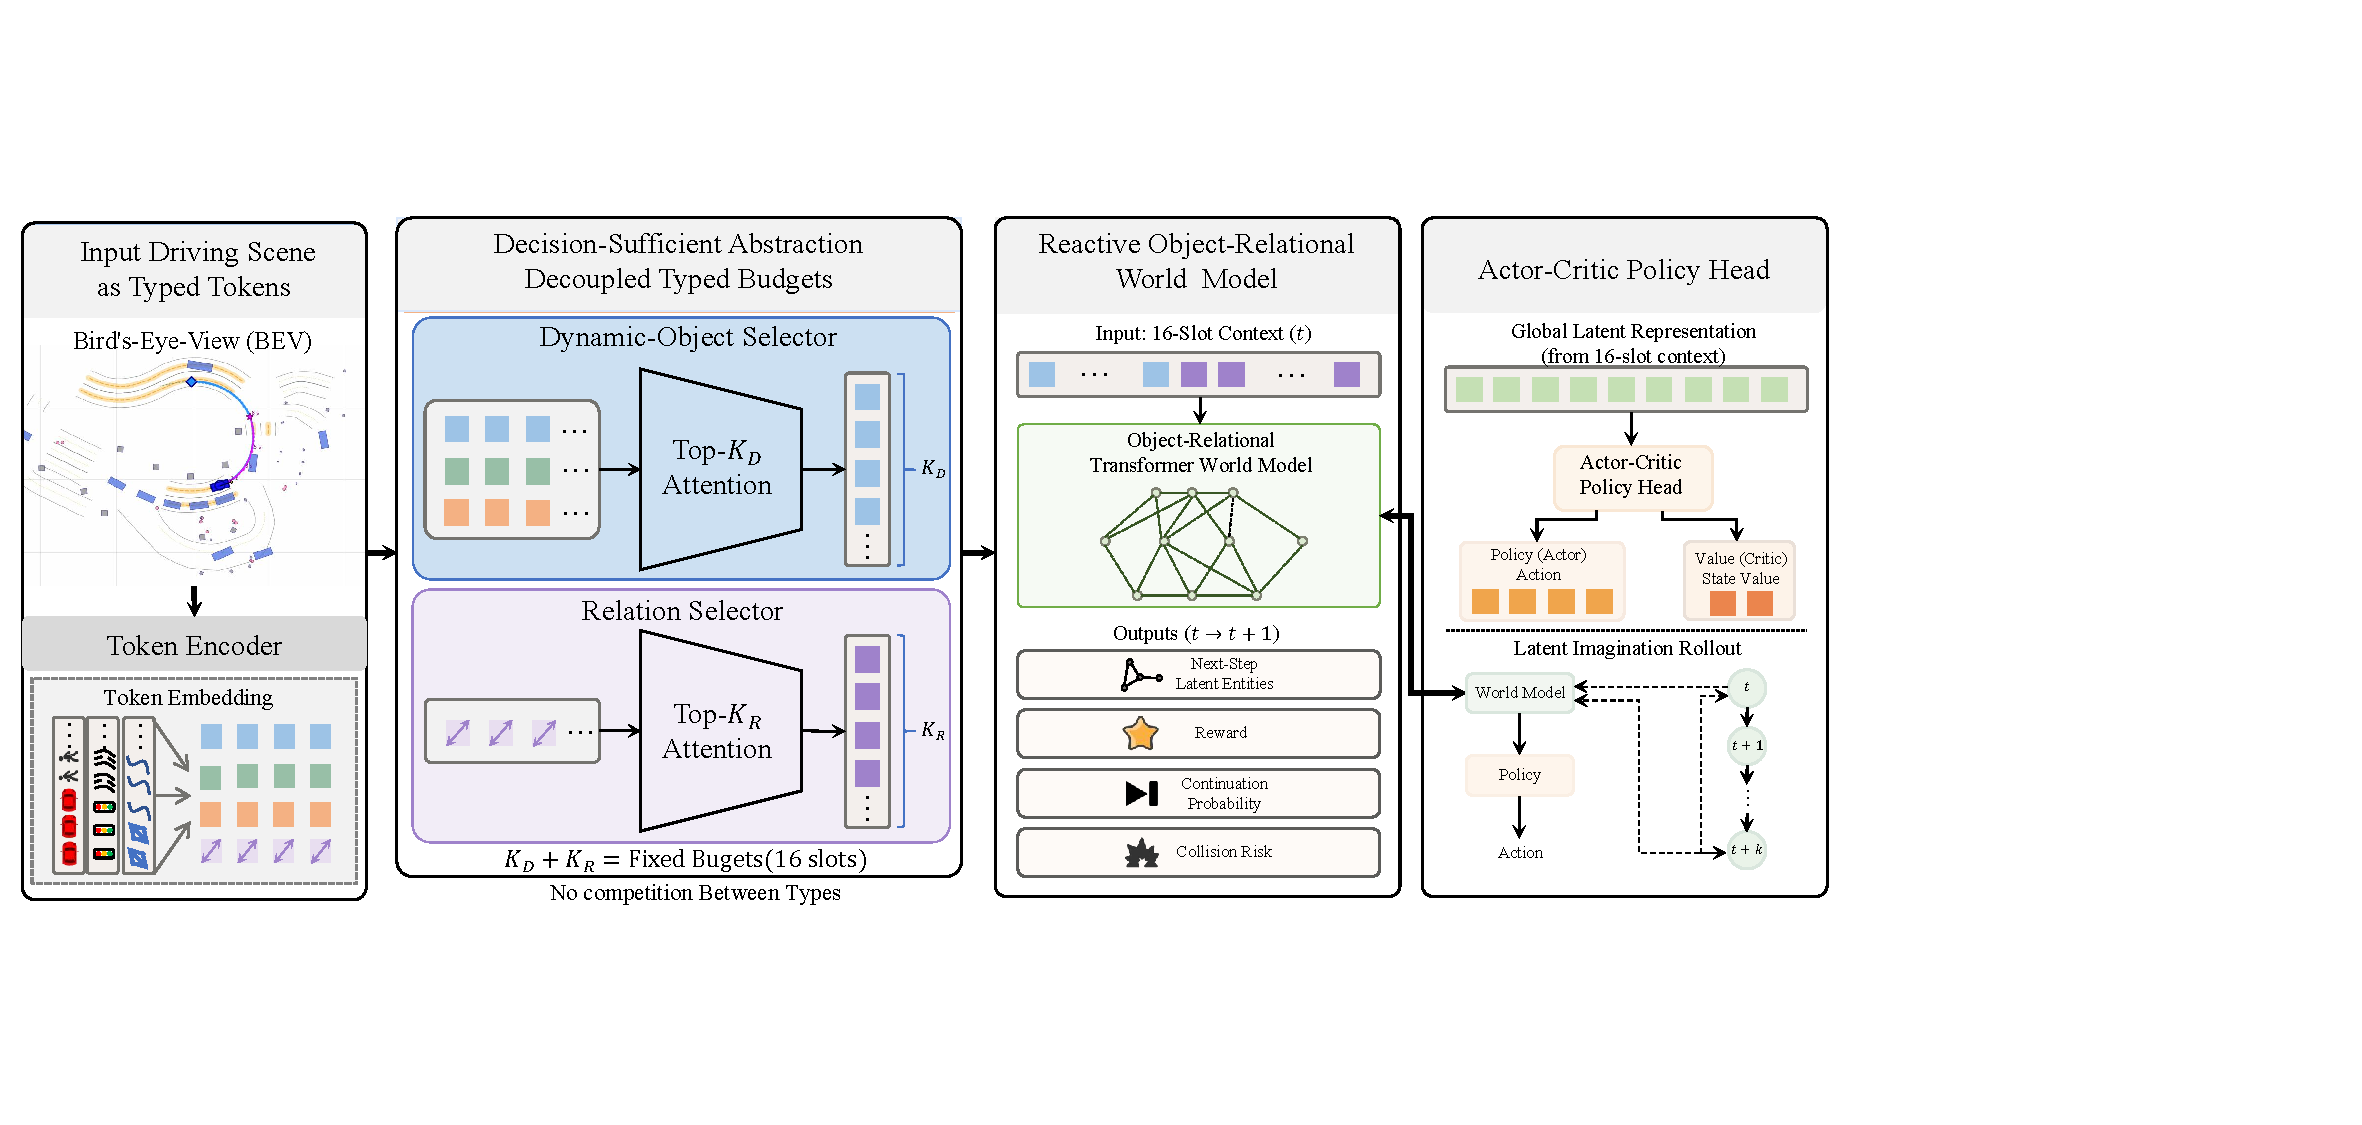
\includegraphics[width=\textwidth]{../figures/fig2.pdf}
\caption{\method\ pipeline. Naive shared-budget selection is compared with typed dyn/rel selection; the fair $(12,4)$ split sits inside the same 16-slot budget, and selected slots feed the action-conditioned world model and policy/value update.}
\label{fig:method_overview}
\end{figure*}

\subsection{Reactive Object-Relational World Model}
The world model receives the selected token set $\mathbf{z}^{\mathrm{sel}}_t$ and action $\mathbf{a}_t$, then predicts next-step latent entities, reward, continuation probability, and collision risk:
\begin{equation}
\hat{\mathbf{z}}^{\mathrm{sel}}_{t+1}, \hat{r}_t, \hat{\rho}_t, \hat{c}_t =
f_\theta(\mathbf{z}^{\mathrm{sel}}_t, \mathbf{a}_t).
\label{eq:worldmodel}
\end{equation}
The action enters the token dynamics, so predicted transitions depend on ego intervention. Without this conditioning, the latent model would behave more like a replay predictor than a reactive model.

The action is projected to the model dimension and prepended as an action token. A two-layer transformer encoder processes the action-token-plus-slot sequence with key padding for masked slots. Transformed non-action slots are decoded to the raw 40-dimensional token space; a masked mean feeds reward, continuation, and collision heads. All fair variants use this world model and differ only in which 16 slots reach it.

The training loss combines next-token prediction, reward prediction, continuation prediction, and auxiliary collision-risk prediction:
\begin{equation}
\mathcal{L}_{\mathrm{wm}} =
\lambda_{\mathrm{obs}}\mathcal{L}_{\mathrm{obs}} +
\lambda_{r}\mathcal{L}_{r} +
\lambda_{\rho}\mathcal{L}_{\rho} +
\lambda_{\mathrm{col}}\mathcal{L}_{\mathrm{col}}.
\label{eq:wmloss}
\end{equation}
The current scaffold also allows an optional behavior-cloning regularizer during warm start,
\begin{equation}
\mathcal{L} = \mathcal{L}_{\mathrm{wm}} + \lambda_{\mathrm{bc}}\mathcal{L}_{\mathrm{bc}} + \mathcal{L}_{\mathrm{pol}},
\label{eq:totalloss}
\end{equation}
which stabilizes early training when the world model and value function are still inaccurate.

The observation loss is type-aware. Dynamic slots, including ego, vehicles, pedestrians, and cyclists, are supervised only on $(x,y,v_x,v_y)$. Relation slots are supervised only on TTC, lane-conflict, and priority fields. Map, signal, and padding slots do not contribute to the next-token observation loss. This avoids forcing relation slots to regress non-physical position or extent targets and aligns the training objective with the representation metrics. For holistic learned-query slots, which no longer correspond to original token indices, we use a set-prediction loss. Each ground-truth dynamic agent is matched to the nearest predicted slot by $(x,y)$, and the loss is applied on the matched $(x,y,v_x,v_y)$ fields. Collision targets are the same for training and evaluation: a sample is positive if any valid relation token has TTC below 3s.

The model still has to learn cross-type dependencies. Relation slots are not decoded in isolation: they pass through the same transformer as dynamic slots, so the predicted next dynamic state can attend to selected relation evidence and the predicted relation fields can attend to selected agent states. The typed budget changes which tokens enter this transformer, not the transformer itself. This distinction is useful for downstream interpretation. If typed budgeting improves Stage-0 dynamic rollout, it suggests that the selected context is more usable by the same dynamics model; if it fails in Stage 1, the bottleneck improvement did not translate into easier policy optimization.

\subsection{Latent Imagination Policy Learning}
Policy and value heads are trained on imagined trajectories from the world model. At each rollout step, the policy head reads $\mathbf{z}^{\mathrm{glob}}_t$ and outputs a diagonal-Gaussian action distribution. The action mean is tanh-bounded and the log standard deviation is clamped before sampling. A value head reads the same global latent. Stage 1 uses a 5-step rollout, GAE-$\lambda$ targets, reward clipping, detached world-model updates, and a real-batch consistency loss. This tests whether the Stage-0 representation gain helps policy learning.

The action schema is two-dimensional: longitudinal velocity along the ego heading and yaw rate. For nuPlan, these are derived from the first future ego pose in the preprocessed NPZ sample; for nuScenes, the adapter uses the available ego-motion or CAN-bus-derived teacher action. During imagination, selected-slot predictions are scattered back into the original 97-slot token layout, non-selected tokens are kept fixed, and the scene is re-encoded before the next abstraction step. This token-space rollout is slower than a pure latent rollout, but it ties Stage 1 to the same encoder and selector used in Stage 0. For learned-query holistic slots, original token identities are unavailable, so the rollout uses a frozen-token approximation; holistic results are therefore treated as secondary checks rather than central evidence.

Stage 1 uses the following shaped reward:
% \vspace{-0.4em}
\begin{equation}
r_t =
w_{\mathrm{prog}} v^{\mathrm{ego}}_{x,t+1}
- w_{\mathrm{coll}}\sigma(\hat{c}_t)
- w_{\mathrm{act}}\|\mathbf{a}_t\|_2^2,
\label{eq:stagereward}
\end{equation}
% \vspace{-0.4em}
with $(w_{\mathrm{prog}},w_{\mathrm{coll}},w_{\mathrm{act}})=(1.0,5.0,0.01)$ and per-step clipping to $[-5,5]$. The world-model reward head is added to this shaped reward, but in offline driving data it contributes weakly because no dense RL reward is available. Policy optimization uses GAE with $(\gamma,\lambda)=(0.97,0.95)$, an entropy term, a Huber critic loss, and a Stage-0 real-batch consistency loss. Stage 1 is a controlled representation-to-policy test, not a new driving reward.

% Algorithm~\ref{alg:doorrl} summarizes the training procedure. Policy improvement stays in latent space, which lets us test whether the abstraction changes downstream policy optimization.

Algorithm~\ref{alg:doorrl} summarizes the training procedure. Policy improvement stays in latent space, letting us test whether the abstraction changes downstream optimization.


\begin{algorithm}[!t]
\caption{\method\ Policy-Learning Procedure}
\label{alg:doorrl}
\begin{algorithmic}[1]
\STATE Collect or load structured scene transitions from offline data and reactive rollouts.
\STATE Encode tokens and compute decision-sufficient latent entities.
\STATE Update the world model using $\mathcal{L}_{\mathrm{wm}}$ in (\ref{eq:wmloss}).
\STATE Warm start the policy with behavior cloning if expert actions are available.
\STATE Roll out imagined latent trajectories with the current policy and world model.
\STATE Update the policy and value heads using imagined rewards, continuation, and value targets.
\STATE Evaluate the policy on the primary held-out validation protocol and supplementary checks.
\STATE Keep the final model according to the paper's primary validation protocol.
\end{algorithmic}
\end{algorithm}

\section{Experimental Setup}
\subsection{Datasets and Protocols}
Table~\ref{tab:protocols} lists the protocols. Stage 0 uses nuScenes for representation analysis under a fair 16-slot world-model budget. Stage 1 reuses the same abstraction family for imagination-based policy learning on nuScenes and on nuPlan preprocessed benchmarks at 20k and 50k scale. The strongest nuPlan condition is then evaluated with an offline planner-like check on the 50k validation split and with interaction-conditioned subsets over lane-conflict, low-TTC, and dense-agent scenes. Cross-dataset rollouts, long-horizon relation interventions, perception-noise probes, and trainable \doorplus\ reliability checks provide mechanism-level evidence. The nuPlan Stage-1 experiments use Stage-0 warm starts trained on the corresponding dataset split.

The nuScenes protocol uses 700 scenes from the trainval split after CAN-bus and invalid-value filtering, yielding 28\,096 tokenized samples. The split is scene-level 80/20, with 560 training scenes and 140 validation scenes, to avoid temporal leakage between train and validation frames from the same scene. For nuPlan, we use preprocessed NPZ samples with a 2-D teacher action derived from the next ego pose: longitudinal velocity along the ego heading and yaw rate over the first 0.1 s future step. The 20k protocol uses a 16k/4k split, and the 50k protocol uses a 40k/10k split. The 50k index is a balanced subset used consistently across the Stage-1 scale-up, planner-like evaluation, relation feature ablation, and interaction-conditioned subset analysis.

All comparisons keep the tokenization, raw feature dimension, world-model architecture, optimizer family, and compact slot budget fixed unless the row explicitly states otherwise. The intent is to compare allocation policies rather than model capacity. The 97-token reference is therefore not treated as a fair competitor; it is an upper-bound check showing what happens when the bottleneck is mostly removed. Likewise, the holistic learned-query model is informative but not central, because it changes token identity and makes relation-aware rollout less direct.

We report averages over seeds whenever repeated runs are available and use the same validation split for all variants inside a protocol. For Stage 0, the primary comparison is the fair 16-slot setting. For Stage 1, the primary comparison is within each dataset-scale block rather than across datasets, because the reward scale and teacher-action distribution differ between nuScenes and nuPlan. Cross-dataset transfer rows are diagnostic: they test whether a warm-started abstraction can survive a dataset shift, but they are not used to claim a universal ranking.

\begin{table}[!t]
\caption{Experimental protocols.}
\label{tab:protocols}
\centering
\resizebox{\columnwidth}{!}{%
\begin{tabular}{lll}
\toprule
Protocol & Dataset and Split & Purpose \\
\midrule
Stage 0 & nuScenes, 700 scenes, 28\,096 samples & Representation sufficiency \\
Stage 1A & nuScenes, 700 scenes, 5\,622 val samples & Short-horizon imagination training \\
Stage 1B & nuPlan 20k, 16k/4k split & Planning-oriented imagination training \\
Stage 1C & nuPlan 50k, 40k/10k split & Scale-up and planner-like evaluation \\
Stage 1D & nuPlan 5k, DOOR $K$ sweep & Capacity-to-policy Pareto study \\
Reliability probes & nuPlan 50k val, 10k/seed & Relation semantics, noise, and \doorplus \\
\bottomrule
\end{tabular}}
\end{table}

\subsection{Variants}
Stage 0 compares six compact 16-slot variants together with one 97-token upper-bound reference:
\begin{enumerate}
\item \textbf{Holistic-16Slot:} learned-query compression from the full token set.
\item \textbf{Object-Only-16:} top-$K$ selection over ego and dynamic-agent tokens only.
\item \textbf{Object+Relation-16:} naive shared-budget top-$K$ over dynamic and relation tokens.
\item \textbf{Object+Relation+Visibility-16:} shared-budget relation-aware selection with visibility weighting.
\item \textbf{Obj+Rel-Decoupled:} typed-budget abstraction with 12 dynamic slots and 4 relation slots.
\item \textbf{Decoupled+Visibility:} typed-budget abstraction plus visibility weighting on the dynamic path.
\end{enumerate}
Stage 1 centers on \texttt{wm\_object}, \texttt{wm\_decoupled}, and \texttt{wm\_decoupled\_no\_vis}. We also report a shared-relation 20k baseline (\texttt{wm\_naive}), a 50k visibility arm (\texttt{wm\_decoupled(+vis)}), a low-cost \texttt{bc} planner-imitation anchor, and two nuScenes-only checks: \texttt{14+2} typed budget and relation-to-critic-only fusion. For the reliability study, \doorplus\ is trained as \texttt{wm\_doorplus\_uncertainty}, warm-started from the typed no-visibility abstraction, with low-confidence false-positive relation augmentation. A post-hoc oracle gate over the DOOR checkpoint is retained only as a diagnostic upper bound.

The Stage-1 names map directly to the Stage-0 abstractions. \texttt{wm\_object} warm-starts from Object-Only-16. \texttt{wm\_decoupled} uses the decoupled typed-budget model with visibility weighting on the dynamic path. \texttt{wm\_decoupled\_no\_vis} uses the same typed-budget split but disables the visibility multiplication. The 20k \texttt{wm\_naive} row warm-starts from the shared Object+Relation abstraction, so it tests whether the shared-relation mechanism remains weak once policy learning is added.

\subsection{Metrics}
Stage 0 reports four representation-centric metrics.
\begin{enumerate}
\item \textbf{Dyn Rollout MSE:} nearest-match squared error on $(x,y,v_x,v_y)$ for dynamic agents.
\item \textbf{Collision F1:} binary F1 of predicted collision risk against labels derived from relation-token time-to-collision below 3 s.
\item \textbf{Rare ADE:} nearest-match displacement error on pedestrians and cyclists.
\item \textbf{Interaction Recall @ 1 m:} fraction of rare agents within 20 m of ego whose nearest-match error is below 1 m.
\end{enumerate}
Stage 1 reports imagination-policy metrics:
\begin{enumerate}
\item \textbf{Return:} $K$-step imagined latent reward sum.
\item \textbf{Collision Rate:} fraction of imagined rollouts whose collision probability exceeds 0.5.
\item \textbf{Collision Mean:} mean of the maximum predicted collision probability over the imagined rollout.
\item \textbf{Ego Stability (cos):} cosine distance between successive ego latents, used to flag liveness and divergence rather than to rank models.
\end{enumerate}
For the nuPlan 50k planner-like evaluation, we also report teacher-action mean-squared error and action $\Delta L_2$ distance. The same Stage-1 metrics are reused for cross-dataset transfer and horizon sensitivity. In the reliability probes, \textbf{Selected-FP-Rel@K} measures the number of artificially injected false-positive relation tokens selected into the relation budget, divided by $K_{\mathrm{rel}}=4$. For example, $0.007$ means that only $0.7\%$ of relation slots are false-positive despite the stress-test candidate density. This mechanism metric tests whether \doorplus\ reduces false-positive relation retention rather than merely changing the collision head output.


\begin{table*}[!t]
\caption{Stage-0 nuScenes representation ablation under a fair 16-slot context budget. Results are averaged over three seeds; $\pm$ is sample standard deviation. Bold marks the best fair-budget result in each metric column. $\Delta$ rows are computed from unrounded run means.}
\label{tab:repr_ablation}
\centering
\resizebox{\textwidth}{!}{%
\begin{tabular}{lccccc}
\toprule
Representation & Ctx & Dyn Rollout $\downarrow$ & Collision F1 $\uparrow$ & Rare ADE $\downarrow$ & IntRec@1m $\uparrow$ \\
\midrule
Holistic-16Slot & 16 & $2.11 \pm 0.16$ & $0.978 \pm 0.011$ & $1.42 \pm 0.01$ & $0.643 \pm 0.015$ \\
Object-Only-16 & 16 & $3.74 \pm 1.01$ & $0.946 \pm 0.004$ & $1.10 \pm 0.12$ & $0.901 \pm 0.034$ \\
Object+Relation-16 (naive) & 16 & $40.28 \pm 29.54$ & $\mathbf{0.980 \pm 0.013}$ & $7.51 \pm 5.48$ & $0.430 \pm 0.407$ \\
Object+Relation+Visibility-16 & 16 & $15.80 \pm 9.93$ & $0.933 \pm 0.064$ & $2.96 \pm 1.64$ & $0.728 \pm 0.155$ \\
\midrule
\textbf{Obj+Rel-Decoupled (Ours)} & 16 & $2.11 \pm 0.19$ & $0.929 \pm 0.039$ & $\mathbf{0.49 \pm 0.18}$ & $\mathbf{0.984 \pm 0.014}$ \\
\textbf{Decoupled+Visibility (Ours)} & 16 & $\mathbf{1.88 \pm 0.23}$ & $0.926 \pm 0.029$ & $0.52 \pm 0.05$ & $0.979 \pm 0.008$ \\
\midrule
$\Delta$ Obj+Rel-Decoupled vs Object-Only & -- & $-43.5\%$ & $-1.8$ pts & $-55.2\%$ & $+8.3$ pts \\
$\Delta$ Decoupled+Vis vs Object-Only & -- & $-49.9\%$ & $-2.1$ pts & $-52.6\%$ & $+7.8$ pts \\
\bottomrule
\end{tabular}}
\end{table*}




For Stage 1, return is the undiscounted sum of the five imagined per-step rewards in (\ref{eq:stagereward}). Collision rate is the fraction of validation rollouts whose maximum predicted collision probability over the horizon exceeds 0.5; collision mean is the mean of that same maximum probability. Ego stability is the mean step-to-step cosine distance of the ego-slot latent over the imagined rollout. The quantity is used as a warning signal rather than a ranking metric: very high values indicate possible latent drift, while very low values can also indicate a collapsed or inactive policy.


\subsection{Implementation Details}
The shared model configuration uses raw token dimension $40$, model dimension $128$, hidden dimension $256$, four attention heads, two transformer world-model layers, dropout $0.1$, and a token budget of $97$. The compact-reference setting uses $K=16$ latent slots, and the capacity-scaling study evaluates $K\in\{16,32,64\}$ with the same tokenization and training protocol. Stage 0 uses Adam with learning rate $10^{-3}$, weight decay $10^{-5}$, batch size $32$, $15$ epochs, and three seeds $\{7,42,123\}$. The Stage-0 loss weights are $\lambda_{\mathrm{obs}}=1.0$, $\lambda_r=0.5$, $\lambda_{\rho}=0.25$, $\lambda_{\mathrm{col}}=0.25$, and $\lambda_{\mathrm{bc}}=0.1$.

Stage 1 uses a 5-step imagination horizon for the main cross-dataset tables, batch size $128$, learning rate $4\times 10^{-3}$, $10$ epochs, three seeds $\{7,42,123\}$, GAE-$\lambda$ targets with $(\gamma,\lambda)=(0.97,0.95)$, reward clipping to $[-5,5]$, a Huber critic with delta 10, a real-batch consistency loss weight of 1.0, and detached world-model dynamics during actor-critic updates. The clean Stage-1 K-scaling study uses the same model family on nuPlan 5k with horizon 10, learning rate $5\times 10^{-4}$, $8$ epochs, and seeds $\{7,42,123\}$ to isolate capacity effects. The diagonal-Gaussian actor uses a tanh-bounded mean in $[-3,3]$, clamps log standard deviation to $[-2,0.5]$, and clips actions during training.


The offline planner-like evaluation is deliberately simple. It does not run a closed-loop simulator or invoke an external planner. Instead, it compares the learned policy action against teacher-derived ego actions on held-out nuPlan samples and reports the same collision-oriented imagination metrics. This makes the check reproducible and tied to the paper's representation question, but it should not be read as a substitute for official nuPlan closed-loop scoring.

\section{Results}
\subsection{Stage-0 Representation Sufficiency on nuScenes}
Table~\ref{tab:repr_ablation} gives the original representation ablation, and Tables~\ref{tab:capacity_scaling}--\ref{tab:budget_sensitivity} extend it into a capacity-regime analysis. The question is no longer whether a single 16-slot split is universally best. Instead, we ask when inter-type competition appears, how quickly it disappears as capacity grows, and which dynamic-versus-relation allocation gives the best compact representation.

Under a 16-slot budget, shared object-relation selection is highly unstable: Dyn Rollout rises to $38.41 \pm 27.90$, Rare ADE to $7.15 \pm 4.79$, and IntRec@1m drops to $0.44 \pm 0.31$. Typed allocation repairs this failure, reducing Dyn Rollout to $0.73 \pm 1.05$, Rare ADE to $0.44 \pm 0.15$, and restoring IntRec@1m to $0.99 \pm 0.02$. Collision F1 tells a different story: holistic and object-only variants can preserve collision proxies while losing interaction recall or rare-agent fidelity. Thus the Stage-0 claim is not all-metric dominance, but decision-sufficient object-relation co-preservation under compact budgets.

\begin{table*}[!t]
\caption{Stage-0 capacity scaling on nuScenes (mean $\pm$ sample standard deviation over three seeds). DOOR gives the clearest compact-budget Pareto gain at $K=16$--$32$; at $K=64$, larger capacity reduces competition and all structured variants approach saturation.}
\label{tab:capacity_scaling}
\centering
\scriptsize
\resizebox{\textwidth}{!}{%
\begin{tabular}{llcccc}
\toprule
$K$ & Variant & Dyn Rollout MSE $\downarrow$ & Rare ADE $\downarrow$ & IntRec@1m $\uparrow$ & Collision F1 $\uparrow$ \\
\midrule
16 & Holistic & $1.963 \pm 0.111$ & $1.430 \pm 0.026$ & $0.619 \pm 0.045$ & $\mathbf{0.985 \pm 0.007}$ \\
16 & Object-only & $4.545 \pm 0.478$ & $1.192 \pm 0.203$ & $0.884 \pm 0.043$ & $0.950 \pm 0.011$ \\
16 & Shared Obj+Rel & $38.411 \pm 27.900$ & $7.147 \pm 4.794$ & $0.441 \pm 0.309$ & $0.939 \pm 0.050$ \\
16 & \textbf{DOOR} & $\mathbf{0.728 \pm 1.046}$ & $\mathbf{0.442 \pm 0.152}$ & $\mathbf{0.990 \pm 0.018}$ & $0.898 \pm 0.017$ \\
\midrule
32 & Holistic & $0.741 \pm 0.112$ & $0.838 \pm 0.147$ & $0.803 \pm 0.071$ & $\mathbf{0.983 \pm 0.005}$ \\
32 & Object-only & $0.589 \pm 0.102$ & $0.433 \pm 0.182$ & $0.979 \pm 0.015$ & $0.957 \pm 0.013$ \\
32 & Shared Obj+Rel & $2.213 \pm 1.583$ & $0.758 \pm 0.378$ & $0.916 \pm 0.053$ & $0.948 \pm 0.030$ \\
32 & \textbf{DOOR} & $\mathbf{0.105 \pm 0.123}$ & $\mathbf{0.235 \pm 0.070}$ & $\mathbf{1.000 \pm 0.000}$ & $0.950 \pm 0.027$ \\
\midrule
64 & Holistic & $0.353 \pm 0.079$ & $0.553 \pm 0.120$ & $0.917 \pm 0.051$ & $0.979 \pm 0.009$ \\
64 & Object-only & $\mathbf{0.096 \pm 0.116}$ & $\mathbf{0.226 \pm 0.079}$ & $\mathbf{1.000 \pm 0.000}$ & $0.964 \pm 0.002$ \\
64 & Shared Obj+Rel & $0.154 \pm 0.090$ & $0.410 \pm 0.289$ & $1.000 \pm 0.000$ & $\mathbf{0.987 \pm 0.005}$ \\
64 & DOOR & $0.123 \pm 0.171$ & $0.289 \pm 0.086$ & $\mathbf{1.000 \pm 0.000}$ & $0.984 \pm 0.006$ \\
\bottomrule
\end{tabular}}
\end{table*}

\begin{table}[!t]
\caption{Approximate slot-attention cost for repeated imagination rollouts. If the recurrent world-model dynamics attends over the selected slots, the dominant slot interaction scales as $O(K^2)$ per rollout step. Larger $K$ can reduce competition, but increases the repeated dynamics cost.}
\label{tab:capacity_cost}
\centering
\resizebox{\columnwidth}{!}{%
\begin{tabular}{lccc}
\toprule
$K$ & Token ratio vs 16 & Slot-attn cost vs 16 & Slot-attn cost vs 32 \\
\midrule
16 & $1.00\times$ & $1.00\times$ & $0.25\times$ \\
32 & $2.00\times$ & $4.00\times$ & $1.00\times$ \\
64 & $4.00\times$ & $16.00\times$ & $4.00\times$ \\
97 & $6.06\times$ & $36.75\times$ & $9.19\times$ \\
\bottomrule
\end{tabular}}
\end{table}

\begin{table*}[!t]
\caption{Stage-0 typed split sensitivity at $K=16$ on nuScenes (mean $\pm$ sample standard deviation over three seeds). Dynamic-heavy 14/2 gives the best dynamic fidelity, rare-agent preservation, and interaction recall; relation-heavy splits can improve collision-proxy F1 but degrade decision-critical object coverage.}
\label{tab:budget_sensitivity}
\centering
\resizebox{\textwidth}{!}{%
\begin{tabular}{lcccc}
\toprule
Split $(K_{\mathrm{dyn}}/K_{\mathrm{rel}})$ & Dyn Rollout MSE $\downarrow$ & Rare ADE $\downarrow$ & IntRec@1m $\uparrow$ & Collision F1 $\uparrow$ \\
\midrule
\textbf{14/2} & $\mathbf{0.089 \pm 0.084}$ & $\mathbf{0.304 \pm 0.103}$ & $\mathbf{1.000 \pm 0.000}$ & $0.909 \pm 0.014$ \\
12/4 & $1.936 \pm 0.387$ & $0.602 \pm 0.183$ & $0.972 \pm 0.015$ & $0.921 \pm 0.038$ \\
10/6 & $9.280 \pm 1.257$ & $2.093 \pm 0.178$ & $0.853 \pm 0.065$ & $\mathbf{0.940 \pm 0.034}$ \\
8/8 & $22.408 \pm 1.738$ & $4.518 \pm 0.470$ & $0.681 \pm 0.131$ & $0.903 \pm 0.041$ \\
\bottomrule
\end{tabular}}
\end{table*}


\begin{table*}[!t]
\caption{Stage-1 imagination-based policy learning across datasets and nuPlan scales. Results are averaged over three seeds where repeated runs are available; $\pm$ is sample standard deviation where shown. Bold numeric entries mark the best return and collision values within each dataset block; bold condition names mark the primary trade-off condition discussed in the text. Ego stability flags divergence and is not the ranking criterion.}
\label{tab:stage1_cross_dataset}
\centering
\resizebox{\textwidth}{!}{%
\begin{tabular}{llcccc}
\toprule
Dataset & Condition & Return $\uparrow$ & Coll. Rate $\downarrow$ & Coll. Mean $\downarrow$ & Ego Stability (cos) \\
\midrule
nuScenes & \textbf{WM-Object} & $\mathbf{31.79 \pm 19.70}$ & $\mathbf{0.597 \pm 0.048}$ & $\mathbf{0.610 \pm 0.048}$ & $0.258 \pm 0.058$ \\
nuScenes & WM-Decoupled & $4.34 \pm 13.66$ & $0.695 \pm 0.283$ & $0.676 \pm 0.243$ & $0.636 \pm 0.108$ \\
nuScenes & WM-Decoupled-NoVis & $0.34 \pm 15.97$ & $0.820 \pm 0.260$ & $0.814 \pm 0.167$ & $0.223 \pm 0.033$ \\
\midrule
nuPlan 20k & WM-Object & $4.74 \pm 13.95$ & $0.373 \pm 0.083$ & $0.395 \pm 0.057$ & $0.426 \pm 0.099$ \\
nuPlan 20k & WM-Naive-Shared & $-2.66 \pm 14.63$ & $0.252 \pm 0.050$ & $0.297 \pm 0.069$ & $0.186$ \\
nuPlan 20k & WM-Decoupled & $13.48 \pm 4.09$ & $0.488 \pm 0.217$ & $0.509 \pm 0.193$ & $0.546 \pm 0.046$ \\
nuPlan 20k & \textbf{WM-Decoupled-NoVis} & $\mathbf{17.50 \pm 1.37}$ & $\mathbf{0.226 \pm 0.105}$ & $\mathbf{0.251 \pm 0.101}$ & $0.136 \pm 0.022$ \\
\midrule
nuPlan 50k & WM-Object & $1.72 \pm 17.89$ & $0.610 \pm 0.146$ & $0.614 \pm 0.113$ & $0.367$ \\
nuPlan 50k & WM-Decoupled(+Vis) & $-0.33 \pm 4.94$ & $\mathbf{0.007 \pm 0.012}$ & $\mathbf{0.277 \pm 0.111}$ & $0.255$ \\
nuPlan 50k & \textbf{WM-Decoupled-NoVis} & $\mathbf{14.51 \pm 2.93}$ & $0.259 \pm 0.045$ & $\mathbf{0.277 \pm 0.033}$ & $0.222$ \\
nuPlan 50k & BC / Planner-Imit. & $0.43 \pm 4.23$ & $0.327 \pm 0.566$ & $0.479 \pm 0.368$ & $0.021$ \\
\bottomrule
\end{tabular}}
\end{table*}


\begin{figure}[!htbp]
\centering
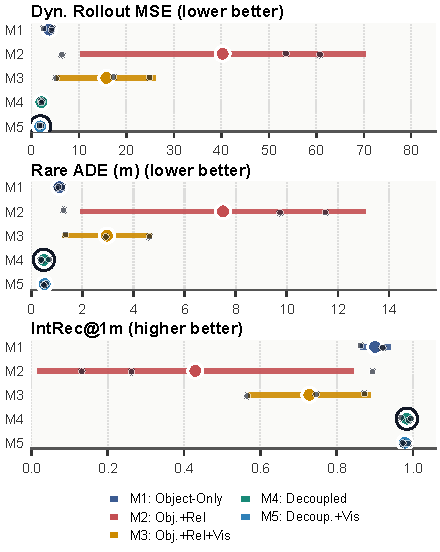
\includegraphics[width=\columnwidth]{../figures/paper_clean/paper_stage0_metrics_clean.pdf}
\caption{Stage-0 nuScenes metrics under the fair 16-slot budget. Typed-budget variants recover dynamic rollout quality, rare-agent fidelity, and interaction recall relative to shared object-relation selection.}
\label{fig:stage0_metrics}
\end{figure}

Naive relation mixing exposes the failure mode. In the three-seed $K=16$ scaling study, Shared Obj+Rel increases Dyn Rollout error to $38.41 \pm 27.90$, increases Rare ADE to $7.15 \pm 4.79$, and drops IntRec@1m to $0.44 \pm 0.31$. The issue is shared-budget competition, not relation structure itself. Fig.~\ref{fig:slot_distribution} shows that shared-budget variants allocate too many slots to relation tokens, while decoupled variants preserve an explicit dynamic-versus-relation split.

\begin{figure}[!t]
\centering
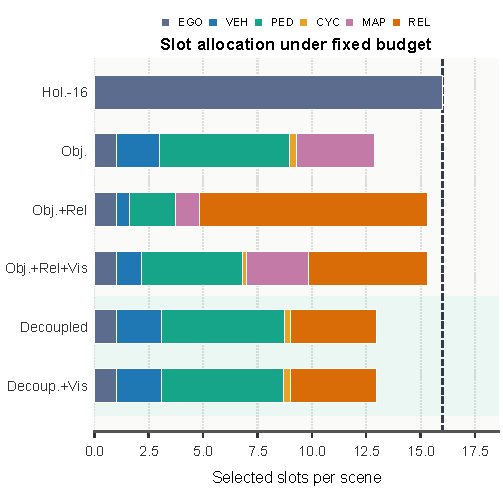
\includegraphics[width=\columnwidth]{../figures/paper_clean/paper_stage0_slot_budget_clean.pdf}
\caption{Stage-0 slot-type composition. Shared object-relation selection over-allocates slots to relation tokens; typed-budget variants preserve dynamic-agent coverage.}
\label{fig:slot_distribution}
\end{figure}

The decoupled variants can lose Collision F1 at very small budgets, especially when the split is optimized for dynamic coverage. In Table~\ref{tab:budget_sensitivity}, 14/2 gives the strongest Dyn, Rare ADE, and IntRec@1m, whereas 10/6 gives the highest Collision F1 but much worse dynamic and rare-agent metrics. This confirms that collision classification alone can favor relation-heavy allocations that preserve collision proxies while discarding decision-critical agent state.

Collision F1 should not be read alone. A model can retain relation-level collision proxies while losing the dynamic-agent slots needed to forecast the interacting entities. For policy learning, a low-TTC relation token only helps if the relevant agents remain in the latent context. The Stage-0 claim is not that typed budgeting maximizes every auxiliary metric, but that it restores joint object-relation structure and exposes the capacity trade-off.


The capacity sweep clarifies why we do not frame DOOR as a replacement for larger contexts. At $K=64$, object-only, shared object-relation, and DOOR all approach saturation on IntRec@1m, and the metric gaps narrow. Larger capacity is therefore a valid but more expensive solution. The value of DOOR is compact-budget Pareto efficiency: it repairs severe shared-selection failures at $K=16$, gives the cleanest dynamic/rare/interaction trade-off at $K=32$, and becomes less decisive once the context is large enough to absorb most token families.


\subsection{Stage-1 Cross-Dataset Imagination Policy Learning}
Stage 0 shows that typed budgeting preserves decision-critical dynamic information under a fixed latent budget. Table~\ref{tab:stage1_cross_dataset} tests whether that representation helps policy optimization on nuScenes short-horizon imagination and nuPlan planning-oriented imagination.

Table~\ref{tab:stage1_cross_dataset} separates two effects. Better representation does not automatically imply better policy learning: on nuScenes, object-only remains the strongest main Stage-1 condition. The nuPlan ranking is different. At 20k, WM-Decoupled-NoVis achieves $17.50 \pm 1.37$ return versus $4.74 \pm 13.95$ for WM-Object and reduces collision rate from $0.373 \pm 0.083$ to $0.226 \pm 0.105$. At 50k, it achieves $14.51 \pm 2.93$ return and $0.259 \pm 0.045$ collision rate versus $1.72 \pm 17.89$ and $0.610 \pm 0.146$ for WM-Object. The WM-Naive-Shared row connects the Stage-0 failure to Stage 1; the BC planner-imitation row gives a non-family reference.

\begin{table*}[!t]
\caption{Clean Stage-1 DOOR capacity Pareto study on nuPlan 5k. The policy experiment uses horizon 10 and three seeds; the measured cost columns come from the matching repeated-rollout benchmark with batch size 128 and horizon 10. $K=32$ is a compact trade-off rather than a global optimum; $K=64$ is stronger downstream but substantially more memory intensive.}
\label{tab:stage1_capacity_pareto}
\centering
\resizebox{\textwidth}{!}{%
\begin{tabular}{lcccccc}
\toprule
$K$ / Split & Return $\uparrow$ & Coll. Rate $\downarrow$ & Coll. Mean $\downarrow$ & H=10 rollout ms & Peak rollout MB & Interpretation \\
\midrule
16 / 14--2 & $-11.96 \pm 7.67$ & $0.815 \pm 0.050$ & $0.811 \pm 0.055$ & $55.6$ & $110.9$ & too constrained \\
32 / 24--8 & $+1.17 \pm 3.36$ & $0.864 \pm 0.036$ & $0.861 \pm 0.032$ & $56.4$ & $166.8$ & compact trade-off \\
64 / 52--12 & $\mathbf{+14.88 \pm 0.78}$ & $\mathbf{0.548 \pm 0.007}$ & $\mathbf{0.556 \pm 0.010}$ & $55.4$ & $288.3$ & stronger but costly \\
\bottomrule
\end{tabular}}
\end{table*}

Table~\ref{tab:stage1_capacity_pareto} adds the missing policy-side capacity check. For DOOR, increasing capacity from $K=16$ to $K=32$ moves the average return from negative to positive, suggesting that the Stage-0 representation improvement can transfer to downstream imagination when the context is no longer severely constrained. However, $K=32$ does not yet deliver the collision stability of $K=64$. The $K=64$ row has the strongest return and collision metrics, which is expected: additional capacity mitigates the bottleneck. The point is not that $K=32$ is optimal, but that it is a compact trade-off, whereas $K=64$ pays substantially higher rollout memory and $O(K^2)$ slot-interaction cost.

Visibility weighting is dataset-dependent. In Stage 0, it slightly improves the best dynamic-rollout metric. In Stage 1, its role changes. On nuScenes, no-visibility is weakest among the three main variants. On nuPlan 20k and 50k, no-visibility has the best return, while the visibility arm behaves more like a collision-suppression extreme. Visibility is not a universal enhancement. Reducing the relation budget from $(12,4)$ to $(14,2)$ does not rescue nuScenes Stage-1 performance, and routing relation information only to the critic gives only partial improvement. The nuScenes gap is therefore not explained by too many relation slots or by a simple actor-versus-critic fusion issue.

\begin{table*}[!t]
\caption{nuScenes Stage-1 ablations under the same 700-scene protocol. Neither a smaller relation budget nor relation-to-critic-only fusion rescues the default decoupled policy.}
\label{tab:nuscenes_aux_ablation}
\centering
\resizebox{\textwidth}{!}{%
\begin{tabular}{lccccc}
\toprule
Condition & Return $\uparrow$ & Coll. Rate $\downarrow$ & Coll. Mean $\downarrow$ & Ego Stability (cos) \\
\midrule
WM-Object & $31.79 \pm 19.70$ & $0.597 \pm 0.048$ & $0.610 \pm 0.048$ & $0.258 \pm 0.058$ \\
WM-Decoupled & $4.34 \pm 13.66$ & $0.695 \pm 0.283$ & $0.676 \pm 0.243$ & $0.636 \pm 0.108$ \\
WM-Decoupled-NoVis & $0.34 \pm 15.97$ & $0.820 \pm 0.260$ & $0.814 \pm 0.167$ & $0.223 \pm 0.033$ \\
WM-Decoupled-14+2 & $2.47 \pm 4.14$ & $0.808 \pm 0.196$ & $0.774 \pm 0.189$ & $0.419 \pm 0.264$ \\
WM-RelToCriticOnly & $5.72 \pm 7.25$ & $0.729 \pm 0.169$ & $0.736 \pm 0.163$ & $0.453 \pm 0.228$ \\
\bottomrule
\end{tabular}}
\end{table*}



The nuPlan warm starts also favor decoupled abstraction. At 20k, object-only yields Dyn Rollout $168.733$ and Rare ADE $17.981$, whereas both decoupled variants reduce these to $3.210$ and $0.848$. At 50k, object-only yields Dyn Rollout $116.627$, Rare ADE $17.318$, and IntRec@1m $0.006$, whereas the decoupled model achieves $2.438$, $0.812$, and $0.914$. The Stage-1 nuPlan gains therefore start from a stronger representation, not from a weaker initialization. Figure~\ref{fig:stage1_cross_dataset_plot} shows the Stage-1 ranking reversal that object-only leads on nuScenes, while WM-Decoupled-NoVis gives the strongest return and fewer collisions than object-only on nuPlan.


\begin{figure}[!t]
\centering
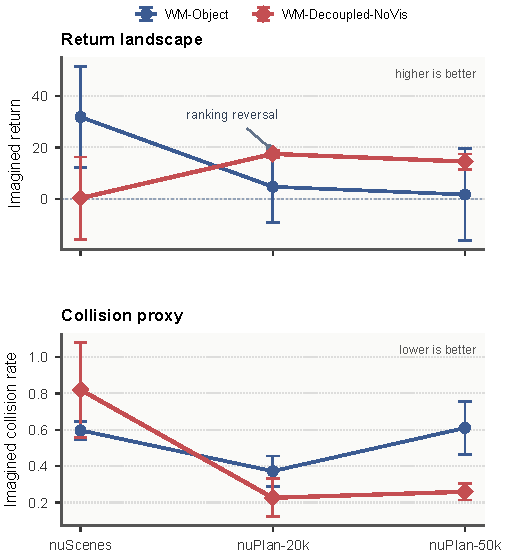
\includegraphics[width=\columnwidth]{../figures/paper_clean/paper_stage1_cross_dataset_clean.pdf}
\caption{Stage-1 cross-dataset evaluation. WM-Object leads on nuScenes, while WM-Decoupled-NoVis has stronger return and lower collision rate than object-only on nuPlan 20k and 50k.}
\label{fig:stage1_cross_dataset_plot}
\end{figure}

\subsection{nuPlan Planner-Like Evaluation}
Table~\ref{tab:planner_sanity} evaluates the two 50k nuPlan finalists with an offline planner-like test. This is not an external closed-loop benchmark. It reuses the nuPlan validation split and measures distance to teacher-derived planner actions while preserving the latent-rollout metrics from Stage 1.

\begin{table*}[!t]
\caption{nuPlan 50k offline planner-like evaluation. Results are averaged over three seeds where repeated runs are available; $\pm$ is sample standard deviation where shown. Lower action error indicates closer agreement with the teacher-derived planner action.}
\label{tab:planner_sanity}
\centering
\resizebox{\textwidth}{!}{%
\begin{tabular}{lccccc}
\toprule
Condition & Teacher Action MSE $\downarrow$ & Action $\Delta L_2$ $\downarrow$ & Return $\uparrow$ & Coll. Rate $\downarrow$ & Progress Proxy $\uparrow$ \\
\midrule
WM-Object & $8.863 \pm 0.370$ & $3.553 \pm 0.118$ & $1.722 \pm 17.888$ & $0.610 \pm 0.146$ & $2.995$ \\
\textbf{WM-Decoupled-NoVis} & $\mathbf{6.628 \pm 0.110}$ & $\mathbf{2.115 \pm 0.083}$ & $\mathbf{14.512 \pm 2.925}$ & $\mathbf{0.259 \pm 0.045}$ & $1.082$ \\
BC / Planner-Imit. & $8.824 \pm 0.113$ & $3.534 \pm 0.017$ & $0.433 \pm 4.229$ & $0.327 \pm 0.566$ & $\mathbf{3.000}$ \\
\bottomrule
\end{tabular}}
\end{table*}

The planner-like evaluation agrees with the 20k/50k Stage-1 tables. WM-Decoupled-NoVis has better latent return and collision metrics and is closer to the teacher-derived action target, reducing action MSE from $8.863$ to $6.628$. The BC / planner-imitation anchor is weaker, with $8.824$ action MSE and much lower return. WM-Object and BC show larger progress proxies, but worse action agreement and collision behavior. This is evidence for the nuPlan ranking, not a benchmark claim.

\begin{table*}[!t]
\caption{nuPlan 50k interaction-conditioned subsets. Each subset isolates scenes where relation reasoning should matter. Values are averaged over three seeds; $\pm$ is sample standard deviation where shown.}
\label{tab:interaction_subsets}
\centering
\resizebox{\textwidth}{!}{%
\begin{tabular}{llccc}
\toprule
Subset & Condition & Teacher Action MSE $\downarrow$ & Return $\uparrow$ & Coll. Rate $\downarrow$ \\
\midrule
lane\_conflict & WM-Object & $7.023 \pm 0.393$ & $0.943 \pm 17.975$ & $0.591 \pm 0.176$ \\
lane\_conflict & \textbf{WM-Decoupled-NoVis} & $\mathbf{4.225 \pm 0.125}$ & $\mathbf{13.330 \pm 3.134}$ & $\mathbf{0.205 \pm 0.043}$ \\
\midrule
low\_ttc\_proxy & WM-Object & $12.796 \pm 0.425$ & $2.650 \pm 18.243$ & $0.791 \pm 0.084$ \\
low\_ttc\_proxy & \textbf{WM-Decoupled-NoVis} & $\mathbf{11.534 \pm 0.198}$ & $\mathbf{15.946 \pm 2.851}$ & $\mathbf{0.541 \pm 0.090}$ \\
\midrule
dense\_agents & WM-Object & $8.692 \pm 0.414$ & $1.423 \pm 17.975$ & $0.637 \pm 0.170$ \\
dense\_agents & \textbf{WM-Decoupled-NoVis} & $\mathbf{6.340 \pm 0.170}$ & $\mathbf{14.311 \pm 3.127}$ & $\mathbf{0.272 \pm 0.049}$ \\
\midrule
rare\_agent\_dense & WM-Object & $8.729 \pm 0.369$ & $1.562 \pm 17.985$ & $0.626 \pm 0.149$ \\
rare\_agent\_dense & \textbf{WM-Decoupled-NoVis} & $\mathbf{6.494 \pm 0.137}$ & $\mathbf{14.496 \pm 3.085}$ & $\mathbf{0.273 \pm 0.045}$ \\
\midrule
high\_interaction\_union & WM-Object & $8.836 \pm 0.410$ & $1.588 \pm 17.940$ & $0.625 \pm 0.150$ \\
high\_interaction\_union & \textbf{WM-Decoupled-NoVis} & $\mathbf{6.555 \pm 0.154}$ & $\mathbf{14.418 \pm 2.994}$ & $\mathbf{0.270 \pm 0.047}$ \\
\bottomrule
\end{tabular}}
\end{table*}

Table~\ref{tab:interaction_subsets} shows where relation-aware abstraction helps. WM-Decoupled-NoVis gains most on subsets where relation structure should matter. In \texttt{lane\_conflict}, action MSE drops from $7.023$ to $4.225$, return rises from $0.943$ to $13.330$, and collision rate falls from $0.591$ to $0.205$. The same direction holds for \texttt{low\_ttc\_proxy}, \texttt{rare\_agent\_dense}, \texttt{dense\_agents}, and their union. Collision rate drops from $0.791$ to $0.541$ on low-TTC scenes and from $0.625$ to $0.270$ on the interaction-heavy union. This subset analysis is more informative than the small closed-loop smoke test because it isolates lane conflict, low TTC, and dense interactive context.

Figure~\ref{fig:planner_subset} visualizes the same downstream pattern without adding a new benchmark. The left side emphasizes that the nuPlan winner is also closer to teacher-derived actions, while the interaction-slice view shows that its collision-rate gain is concentrated where relation information should be most useful. Figure~\ref{fig:qualitative} gives a complementary scene-level view: typed budgeting does not simply add relation slots; it preserves near-field dynamic coverage while reserving a small number of high-risk relation slots. Together, the two figures connect the aggregate policy result to the underlying slot-allocation mechanism.

\begin{figure}[!t]
\centering
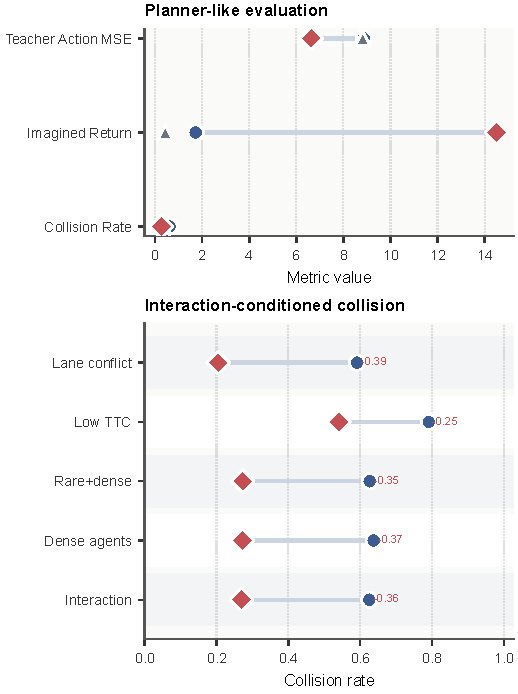
\includegraphics[width=\columnwidth]{../figures/paper_clean/paper_planner_subset_clean.pdf}
\caption{nuPlan 50k offline evidence. WM-Decoupled-NoVis is closer to the teacher-derived action target and gains more on interaction-conditioned subsets.}
\label{fig:planner_subset}
\end{figure}

\begin{figure}[!t]
\centering
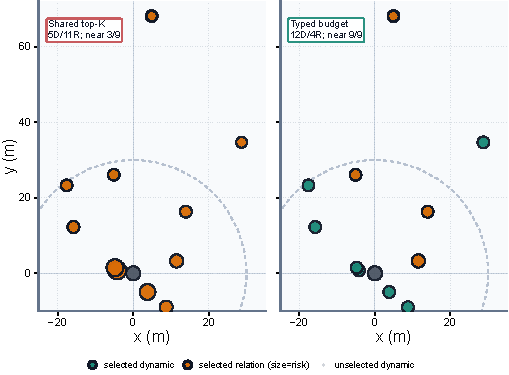
\includegraphics[width=\columnwidth]{../figures/paper_clean/paper_qualitative_slot_selection_3d.pdf}
\caption{Qualitative slot-selection case under the fair 16-slot budget. Bird's-eye coordinates show ego-centric token positions; all markers use the same circular shape, color denotes selected dynamic versus selected relation tokens, and relation-marker size encodes normalized interaction risk. Typed-budget selection keeps more near-field dynamic agents while reserving a small relation budget.}
\label{fig:qualitative}
\end{figure}

\begin{table}[!t]
\caption{Dataset statistics for the Stage-1 ranking reversal. Values are computed from the tokenized validation protocols.}
\label{tab:dataset_stats}
\centering
\resizebox{\columnwidth}{!}{%
\begin{tabular}{lcc}
\toprule
Statistic & nuScenes & nuPlan 50k \\
\midrule
Dynamic tokens / sample & $9.715$ & $12.164$ \\
Rare tokens / sample & $2.439$ & $3.934$ \\
Map tokens / sample & $9.440$ & $31.768$ \\
Relation tokens / sample & $11.318$ & $11.164$ \\
Dynamic visibility mean & $0.746$ & $1.000$ \\
Teacher action $L_2$ mean & $0.539$ & $3.420$ \\
Relation lane-conflict mean & $0.111$ & $0.116$ \\
\bottomrule
\end{tabular}}
\end{table}

\subsection{Relation Semantics, Perception-Noise Robustness, and Trainable DOOR+}

\begin{table*}[!t]
\caption{nuPlan 50k relation feature-group ablation on trained WM-Decoupled-NoVis checkpoints. The ablation is applied at evaluation time, without retraining; small differences between the full model and no-lane-priority rows are within noise.}
\label{tab:relation_groups}
\centering
\resizebox{\textwidth}{!}{%
\begin{tabular}{llcccccc}
\toprule
Condition & Ablation & Teacher MSE $\downarrow$ & Action $\Delta L_2$ $\downarrow$ & Return $\uparrow$ & Coll. Rate $\downarrow$ & Coll. Mean $\downarrow$ & Stability \\
\midrule
WM-Decoupled-NoVis & none & $6.628 \pm 0.110$ & $2.115 \pm 0.083$ & $14.510 \pm 2.921$ & $0.260 \pm 0.045$ & $0.277 \pm 0.033$ & $0.222$ \\
WM-Decoupled-NoVis & no\_ttc\_risk & $7.992 \pm 0.805$ & $3.154 \pm 0.335$ & $8.498 \pm 1.397$ & $0.895 \pm 0.126$ & $0.891 \pm 0.126$ & $0.222$ \\
WM-Decoupled-NoVis & no\_lane\_priority & $6.627 \pm 0.111$ & $2.113 \pm 0.081$ & $14.526 \pm 2.931$ & $0.257 \pm 0.052$ & $0.274 \pm 0.040$ & $0.222$ \\
WM-Decoupled-NoVis & no\_relation\_semantics & $7.989 \pm 0.827$ & $3.151 \pm 0.351$ & $8.724 \pm 1.629$ & $0.894 \pm 0.126$ & $0.888 \pm 0.127$ & $0.222$ \\
\bottomrule
\end{tabular}}
\end{table*}

\begin{table*}[!t]
\caption{Long-horizon relation-semantic interventions on nuPlan 50k WM-Decoupled-NoVis checkpoints. The intervention is evaluation-only. Removing TTC/risk semantics sharply increases collision over 10, 20, and 50-step imagination, while removing lane/priority is nearly neutral.}
\label{tab:long_relation_semantics}
\centering
\resizebox{\textwidth}{!}{%
\begin{tabular}{llcccc}
\toprule
Horizon & Ablation & Return $\uparrow$ & Coll. Rate $\downarrow$ & Coll. Mean $\downarrow$ & Teacher MSE $\downarrow$ \\
\midrule
10 & none & $33.746 \pm 7.209$ & $0.260 \pm 0.045$ & $0.277 \pm 0.033$ & $6.628 \pm 0.110$ \\
10 & no\_ttc\_risk & $27.475 \pm 5.710$ & $0.895 \pm 0.126$ & $0.891 \pm 0.126$ & $7.992 \pm 0.805$ \\
10 & no\_lane\_priority & $33.755 \pm 7.239$ & $0.257 \pm 0.052$ & $0.274 \pm 0.040$ & $6.627 \pm 0.111$ \\
\midrule
20 & none & $72.241 \pm 16.020$ & $0.260 \pm 0.045$ & $0.277 \pm 0.033$ & $6.628 \pm 0.110$ \\
20 & no\_ttc\_risk & $65.535 \pm 14.464$ & $0.896 \pm 0.126$ & $0.891 \pm 0.126$ & $7.992 \pm 0.805$ \\
20 & no\_lane\_priority & $72.231 \pm 16.064$ & $0.257 \pm 0.052$ & $0.274 \pm 0.040$ & $6.627 \pm 0.111$ \\
\midrule
50 & none & $187.733 \pm 42.602$ & $0.260 \pm 0.045$ & $0.277 \pm 0.033$ & $6.628 \pm 0.110$ \\
50 & no\_ttc\_risk & $179.790 \pm 40.690$ & $0.896 \pm 0.126$ & $0.891 \pm 0.126$ & $7.992 \pm 0.805$ \\
50 & no\_lane\_priority & $187.724 \pm 42.610$ & $0.257 \pm 0.052$ & $0.274 \pm 0.040$ & $6.627 \pm 0.111$ \\
\bottomrule
\end{tabular}}
\end{table*}

\begin{table*}[!t]
\caption{Perception-noise robustness and trainable \doorplus\ reliability on nuPlan 50k. DOOR exposes the residual failure mode: high-risk false-positive relation tokens can occupy reserved relation slots. The post-hoc oracle gate is a diagnostic upper bound. The trainable \doorplus\ confidence-token selector is the main method: even when false-positive candidate density is high, it selects almost no false-positive relation slots and preserves clean-level return with only minor collision degradation under relfp0.2.}
\label{tab:doorplus_noise}
\centering
\resizebox{\textwidth}{!}{%
\begin{tabular}{lclcccccc}
\toprule
Condition & Horizon & Perturbation & Return $\uparrow$ & Coll. Rate $\downarrow$ & Coll. Mean $\downarrow$ & Teacher MSE $\downarrow$ & Selected-FP-Rel@K $\downarrow$ & FP density/K \\
\midrule
WM-Object & 10 & clean & $1.922 \pm 41.820$ & $0.676 \pm 0.095$ & $0.673 \pm 0.062$ & $8.863 \pm 0.370$ & -- & -- \\
WM-Object & 10 & relfp0.2 & $1.918 \pm 41.833$ & $0.676 \pm 0.096$ & $0.673 \pm 0.063$ & $8.863 \pm 0.370$ & -- & -- \\
WM-Naive-Shared & 10 & clean & $-5.998 \pm 11.006$ & $0.415 \pm 0.521$ & $0.450 \pm 0.239$ & $8.912 \pm 0.245$ & -- & -- \\
WM-Naive-Shared & 10 & relfp0.2 & $-6.012 \pm 10.996$ & $0.416 \pm 0.521$ & $0.453 \pm 0.236$ & $8.921 \pm 0.259$ & -- & -- \\
\midrule
DOOR & 10 & clean & $33.758 \pm 7.204$ & $0.260 \pm 0.045$ & $0.277 \pm 0.033$ & $6.628 \pm 0.110$ & $0.000$ & $0.000$ \\
DOOR & 10 & loc1.5 & $33.735 \pm 7.215$ & $0.262 \pm 0.045$ & $0.280 \pm 0.033$ & $6.628 \pm 0.110$ & $0.000$ & $0.000$ \\
DOOR & 10 & miss0.2 & $30.567 \pm 5.529$ & $0.247 \pm 0.033$ & $0.260 \pm 0.023$ & $6.633 \pm 0.115$ & $0.000$ & $0.000$ \\
DOOR & 10 & relfp0.2 & $32.847 \pm 6.921$ & $0.457 \pm 0.126$ & $0.469 \pm 0.116$ & $6.727 \pm 0.250$ & $0.150 \pm 0.074$ & $0.556$ \\
\midrule
\doorplus\ posthoc diagnostic & 10 & relfp0.2 & $33.793 \pm 7.236$ & $0.242 \pm 0.046$ & $0.261 \pm 0.032$ & $6.627 \pm 0.110$ & $0.111 \pm 0.018$ & $0.556$ \\
\midrule
\doorplus\ trainable & 20 & clean & $47.299 \pm 19.360$ & $0.953 \pm 0.013$ & $0.905 \pm 0.015$ & $6.839 \pm 0.243$ & $0.000$ & $0.000$ \\
\doorplus\ trainable & 20 & relfp0.2 & $47.394 \pm 19.551$ & $0.967 \pm 0.008$ & $0.916 \pm 0.014$ & $6.815 \pm 0.226$ & $0.007 \pm 0.000$ & $0.556$ \\
\doorplus\ trainable & 50 & clean & $143.913 \pm 34.885$ & $0.953 \pm 0.013$ & $0.905 \pm 0.015$ & $6.839 \pm 0.243$ & $0.000$ & $0.000$ \\
\doorplus\ trainable & 50 & relfp0.2 & $144.027 \pm 35.502$ & $0.967 \pm 0.008$ & $0.916 \pm 0.014$ & $6.815 \pm 0.226$ & $0.007 \pm 0.000$ & $0.556$ \\
\bottomrule
\end{tabular}}
\end{table*}

\begin{table}[!t]
\caption{Long-horizon confirmation for trainable \doorplus\ under false-positive relation noise. Selected-FP-Rel@K remains near zero across horizons despite high false-positive candidate density.}
\label{tab:doorplus_long}
\centering
\resizebox{\columnwidth}{!}{%
\begin{tabular}{lccccc}
\toprule
Horizon & clean Return & relfp Return & clean Coll. & relfp Coll. & Selected-FP-Rel@K \\
\midrule
10 & $20.626$ & $20.669$ & $0.953$ & $0.967$ & $0.007$ \\
20 & $47.299$ & $47.394$ & $0.953$ & $0.967$ & $0.007$ \\
50 & $143.913$ & $144.027$ & $0.953$ & $0.967$ & $0.007$ \\
\bottomrule
\end{tabular}}
\end{table}

Tables~\ref{tab:long_relation_semantics}--\ref{tab:doorplus_long} turn the relation analysis into a failure-and-repair study. First, relation utility is not diffuse across all relation fields. Masking TTC/risk increases collision rate from about $0.26$ to about $0.90$ at horizons 10, 20, and 50, whereas masking lane-conflict/priority is nearly neutral. This identifies the dominant semantic channel used by the nuPlan relation pathway. Second, evaluation-time noise probes show that the typed-budget model is stable under localization noise and random token misses, but high-risk false-positive relation tokens remain harmful. Third, a post-hoc oracle reliability gate sharply reduces relfp0.2 collision, confirming that relation-slot contamination is the cause rather than general model instability. Finally, trainable \doorplus\ reproduces the reliability mechanism without oracle filtering. Although more than half of the relation candidate density is false-positive under the relfp0.2 stress setting (FP density/K $=0.556$), the trainable confidence-token selector selects only $0.007$ false-positive relation slots per $K_{\mathrm{rel}}$ across horizons 10, 20, and 50, while maintaining clean-to-noisy return. We deliberately interpret this as relation-selection reliability, not as evidence that \doorplus\ is a universal policy-improvement module.

\subsection{Does DOOR+ Really Use Relation Confidence?}

Table~\ref{tab:doorplus_confidence_ablation} tests whether \doorplus\ improves because it uses relation confidence, rather than because it adds another selector variant or simply suppresses all relation evidence. We hold the relfp0.2 input density nearly fixed and perturb only the confidence assignment seen by the trainable selector. With the correct confidence-token alignment, selected false-positive occupancy is $0.008 \pm 0.002$, while selected non-FP true-risk occupancy is $0.083 \pm 0.013$ out of a true-risk candidate density of $0.139$. Shuffling confidence across relation candidates or setting all relation confidence to a constant raises selected false-positive occupancy to roughly $0.12$ and lowers true-risk occupancy. Inverting confidence makes false positives look reliable and true relation candidates look unreliable; selected false-positive occupancy then rises to $0.536 \pm 0.010$, nearly matching the FP density/K of $0.558$, while true-risk occupancy drops to $0.043 \pm 0.007$. Thus the mechanism follows a clear causal gradient: the selector routes relation capacity according to confidence quality, not merely according to added parameters or random regularization.

\begin{table}[!t]
\caption{Confidence and true-risk retention ablation for trainable \doorplus\ on nuPlan 50k relfp0.2, horizon 20 (2k validation samples per seed). FP and true-risk candidate densities remain nearly fixed, but the selected relation-slot composition changes sharply with confidence quality.}
\label{tab:doorplus_confidence_ablation}
\centering
\resizebox{\columnwidth}{!}{%
\begin{tabular}{lcccc}
\toprule
Confidence setting & Selected-FP-Rel@K $\downarrow$ & FP density/K & Selected-TrueRisk-Rel@K $\uparrow$ & TrueRisk density/K \\
\midrule
normal & $0.008 \pm 0.002$ & $0.558$ & $0.083 \pm 0.013$ & $0.139$ \\
shuffled & $0.123 \pm 0.030$ & $0.557$ & $0.067 \pm 0.007$ & $0.137$ \\
constant & $0.117 \pm 0.033$ & $0.558$ & $0.073 \pm 0.010$ & $0.139$ \\
inverted & $0.536 \pm 0.010$ & $0.558$ & $0.043 \pm 0.007$ & $0.139$ \\
\bottomrule
\end{tabular}}
\end{table}

\begin{table*}[!t]
\caption{Cross-dataset transfer and horizon sensitivity. Transfer rows report mean $\pm$ sample standard deviation over three seeds. Horizon rows come from the synchronized nuScenes sweep.}
\label{tab:support_diagnostics}
\centering
\resizebox{\textwidth}{!}{%
\begin{tabular}{llcccc}
\toprule
Setting & Condition & Return $\uparrow$ & Coll. Rate $\downarrow$ & Ego-cos step $\downarrow$ & Max action norm \\
\midrule
nuScenes $\rightarrow$ nuPlan & WM-Object & $27.18 \pm 11.44$ & $0.593 \pm 0.261$ & $0.369 \pm 0.203$ & -- \\
nuScenes $\rightarrow$ nuPlan & WM-Decoupled(+Vis) & $-1.43 \pm 17.28$ & $0.593 \pm 0.320$ & $0.853 \pm 0.102$ & -- \\
nuPlan $\rightarrow$ nuScenes & WM-Object & $5.51 \pm 11.65$ & $0.624 \pm 0.135$ & $0.301 \pm 0.154$ & -- \\
nuPlan $\rightarrow$ nuScenes & \textbf{WM-Decoupled-NoVis} & $\mathbf{16.07 \pm 2.20}$ & $\mathbf{0.434 \pm 0.045}$ & $\mathbf{0.181 \pm 0.039}$ & -- \\
\midrule
nuScenes $H=3$ & WM-Object & $11.856$ & $0.570$ & $0.296$ & $3.781$ \\
nuScenes $H=3$ & WM-Decoupled & $1.646$ & $0.683$ & $0.710$ & $4.056$ \\
nuScenes $H=5$ & WM-Object & $21.814$ & $0.603$ & $0.190$ & $3.846$ \\
nuScenes $H=5$ & WM-Decoupled & $-1.462$ & $0.838$ & $0.725$ & $4.205$ \\
nuScenes $H=7$ & WM-Object & $31.950$ & $0.610$ & $0.143$ & $3.850$ \\
nuScenes $H=7$ & WM-Decoupled & $-5.914$ & $0.916$ & $0.733$ & $4.209$ \\
\bottomrule
\end{tabular}}
\end{table*}


Cross-dataset transfer and horizon sweeps give the same picture. In pure cross-dataset rollout evaluation, a nuScenes-trained WM-Decoupled(+Vis) policy transfers poorly to nuPlan, dropping to $-1.43$ mean return with ego-step drift $0.853$. In the opposite direction, a nuPlan-trained WM-Decoupled-NoVis policy transfers to nuScenes better than a nuPlan-trained WM-Object policy, improving return from $5.51$ to $16.07$ and reducing collision rate from $0.624$ to $0.434$. In a nuScenes horizon sweep, the decoupled collision gap grows from $+0.113$ at rollout horizon $H=3$ to $+0.306$ at $H=7$. These checks point to compounding imagination drift on nuScenes, while the nuPlan gain survives transfer and interaction-focused slices. An oracle-token planner wrapper was also connected to the official nuPlan simulation path as an integration smoke test, but that small closed-loop run is not used as main evidence because wrapper feasibility dominates the outcome.

The dataset statistics in Table~\ref{tab:dataset_stats}, relation-feature ablation in Table~\ref{tab:relation_groups}, and transfer diagnostics in Table~\ref{tab:support_diagnostics} provide the mechanism-level support for this interpretation.


\section{Discussion}
The experiments separate representation quality from policy utility, revealing that relation tokens are not universally beneficial. The main capacity result is now sharper: capacity matters twice. Stage 0 shows that capacity first controls representation sufficiency. Typed budgeting is most valuable in compact and medium contexts where shared top-$K$ selection creates inter-type competition, while at larger $K$ the gap narrows as all methods approach saturation. Stage 1 shows that capacity also controls downstream imagination-policy utility. In the clean DOOR K-scaling study, moving from $K=16$ to $K=32$ changes return from negative to positive, and $K=64$ gives the strongest return and collision metrics. This does not contradict the compact-budget claim. Rather, it confirms that object-relation competition is a capacity-dependent phenomenon: increasing $K$ can mitigate the bottleneck, but doing so increases repeated-rollout memory and slot-interaction cost.

These findings challenge the common assumption that adding pairwise interaction features monotonically enriches the scene state. Under a bounded latent bottleneck, a relation feature can be harmful if it crowds out the agent state needed for action-conditioned prediction. Typed budgeting addresses this by enforcing an explicit and diagnosable capacity policy rather than relying on a shared top-$K$ pool or hand-crafted distance rules. The split sweep shows that this policy is not a fixed 12/4 prescription: for nuScenes Stage 0, a dynamic-heavy 14/2 split is best for dynamic fidelity, rare-agent preservation, and interaction recall, while relation-heavy splits can improve collision-proxy F1 at the cost of losing decision-critical objects. The K-scaling results further clarify how to use the method. $K=16$ is too constrained for stable downstream policy utility, even when the representation mechanism is correct. $K=32$ is a compact trade-off point: it improves return relative to $K=16$ but does not yet deliver the collision stability of $K=64$. $K=64$ is stronger downstream, but it is not a free replacement for compact models because the rollout memory rises substantially. This makes the object-relational abstraction a useful intermediate representation between perception and planning, where strict latency and memory budgets demand a compact yet descriptive scene state.

The reliability probes refine this picture. Typed budgeting should not be described as uniformly robust to perception noise. It is stable under the controlled localization and missing-token perturbations used here, but it remains sensitive to false-positive high-risk relation tokens because those tokens occupy the relation slots that \method\ deliberately reserves. This is not a contradiction; it separates two levels of the abstraction problem. \method\ solves inter-type budget competition, while \doorplus\ addresses intra-relation reliability failure. The post-hoc gate serves as a diagnostic upper bound showing that penalizing low-confidence high-risk relations can repair the false-positive failure mode. The trainable confidence-token selector then turns that diagnosis into a deployable reliability mechanism: it substantially mitigates relation-slot contamination from false positives while preserving the typed dynamic-agent budget. The confidence ablation is important because it rules out the simplest alternative explanation. When confidence is shuffled or held constant, false positives re-enter selected slots; when confidence is inverted, selected false-positive occupancy nearly matches the false-positive candidate density. At the same time, normal confidence retains more non-FP true-risk relations than the corrupted-confidence settings. We do not use \doorplus\ as the Stage-1 K-scaling method. A same-setting K32 pilot showed that directly coupling trainable uncertainty gating with larger-capacity Stage-1 policy/world-model optimization can be unstable, whereas the clean DOOR baseline remains usable. This negative result is consistent with the broader finding that improved representation or selection reliability does not automatically translate into policy gains without a matching optimization objective.

The study has several limitations that motivate future work. First, the core training protocol still relies on oracle tokens; \doorplus\ makes relation selection confidence-aware, but the confidence values are injected or supplied as token fields rather than produced by a full detector-integrated stack. Second, the policy claims rest on imagination-based training rather than large-scale closed-loop deployment. Future iterations must connect this typed abstraction to official simulator protocols with matched controller logic. Third, measured wall-clock latency in our synthetic rollout benchmark is partly masked by hardware parallelism, so the cost argument should be read together with peak rollout memory and the theoretical $O(K^2)$ slot-interaction scaling. Fourth, the role of visibility remains unresolved, acting variably as an enhancement, a stabilizer, or a liability depending on the dataset. Finally, the best typed split is dataset- and metric-dependent. The current work makes this dependency explicit; a natural extension is adaptive budgeting, where the model predicts scene-conditioned $K_{\mathrm{dyn}}(x)$ and $K_{\mathrm{rel}}(x)$ under a fixed total $K$ and a global latency constraint.



% The experiments separate representation quality from policy utility. Stage 0 shows that typed budgeting improves decision-sufficient structure under a fixed latent budget. Stage 1 shows that this does not guarantee policy gains. On nuScenes short-horizon imagination, object-only remains strongest. On nuPlan 20k/50k, the no-visibility decoupled variant gives the strongest return and lowers imagined collision metrics relative to object-only, and both the planner-like evaluation and the interaction-conditioned subsets match that ranking. Relation tokens are neither universally helpful nor useless; their value depends on the data and task.

% The cross-dataset ranking reversal is consistent with Tables~\ref{tab:dataset_stats}--\ref{tab:support_diagnostics}. nuPlan has denser dynamic context, more vulnerable road users, nearly constant visibility, and a much larger teacher-action scale. These differences make relation structure easier to use in nuPlan imagination and make visibility weighting less informative. In nuScenes Stage 1, relation information may be harder to exploit because the short-horizon latent objective, smaller ego-motion scale, and actor dynamics favor a simpler dynamic-only policy. In nuPlan 20k/50k, planning-oriented tokens let the decoupled abstraction turn representation gains into policy gains. The relation feature-group ablation gives a more specific mechanism: masking TTC/risk semantics sharply degrades return and collision behavior, while masking lane-conflict/priority is nearly neutral.

% The results also clarify what the method is not doing. Typed budgeting is not merely adding relation tokens. The shared object-relation baseline already adds them, yet it can perform worse because relation tokens compete with dynamic agents. The method is also not simply favoring nearby agents through a hand-crafted distance rule. Dynamic selection remains learned, and the qualitative case in Fig.~\ref{fig:qualitative} shows that the typed split changes which near-field agents survive the bottleneck while keeping a small relation inventory. The benefit therefore comes from preserving complementary token families under one fixed capacity.

% The nuScenes Stage-1 result is useful because it is a negative result for the strongest version of the claim. If relation-aware typed budgeting automatically improved policy learning, the decoupled variants would dominate after the Stage-0 gain. They do not. This suggests that relation information can make the latent state more predictive without making the actor update easier. Short-horizon imagination, noisy teacher actions, and small ego-motion scale may all favor a representation that is simpler for the policy head. In that setting, relation tokens may help the model explain the scene while adding variance to the actor input.

% The nuPlan result points in the opposite direction. The planning-oriented tokenization has denser dynamic context and larger teacher-action variation, and the interaction-conditioned subsets directly stress relation semantics. There, the no-visibility typed-budget variant is consistently strongest on return-oriented comparisons. The visibility reversal is especially informative. Visibility weighting is a plausible prior for nuScenes because visibility varies across annotations, but it becomes nearly constant or uninformative in the nuPlan preprocessing. A feature that is helpful as a dataset-specific confidence signal can become a distracting scale factor when transferred to another protocol.

% These observations argue for treating object-relational abstraction as a dataset- and task-conditioned design choice. A fixed bottleneck should not be judged only by aggregate forecasting error, and a policy result should not be interpreted without checking which token families the abstraction preserves. The two-stage protocol is useful because it exposes both sides: Stage 0 asks whether the representation is sufficient, and Stage 1 asks whether the policy can exploit that sufficiency. This separation also makes negative results interpretable. The nuScenes policy result does not contradict the representation result; it identifies a regime where the actor is not helped by the additional relation structure under the current imagination objective.

% The practical implication is that relation modeling should be introduced with an explicit capacity policy. In many driving stacks, adding pairwise interaction features is treated as a monotonic enrichment of the scene state. Our results show that this is not true once the world model has a fixed number of latent slots. A relation feature can be correct and still be harmful if it occupies the slot that would otherwise carry the agent state needed for action-conditioned prediction. Typed budgeting is a simple way to make that trade-off inspectable: dynamic coverage, relation coverage, and downstream policy utility can be measured separately rather than collapsed into one aggregate forecasting score.

% The results also suggest how the method should be used in a larger autonomy stack. The typed abstraction is most appropriate as an intermediate representation module between perception/prediction and planning, where latency and memory budgets require a compact scene state. It defines which small subset of an already structured scene should be exposed to a world model and a policy head. This makes the method compatible with stronger front-ends as long as token type and relation semantics remain explicit.

% The study has several limitations. First, it assumes oracle-token evaluation, so the results do not include perception noise. Second, Stage 1 is an imagination-based policy study, not a large external closed-loop benchmark; the policy claims are representation-to-policy evidence, not deployment validation. Official nuPlan closed-loop simulation was connected through an oracle-token planner wrapper, but wrapper quality still dominates the outcome, so those runs are not main evidence. Third, visibility remains unresolved: it is a weak Stage-0 enhancement, a nuScenes Stage-1 stabilizer, and a nuPlan Stage-1 liability. Finally, the paper does not yet include a competitive external benchmark table under fully matched metrics.

% Several extensions follow directly from these limitations. The first is perception-aware evaluation, where token uncertainty and missed detections are passed into the abstraction module rather than removed by oracle tokens. The second is adaptive budgeting: instead of fixing $(12,4)$ for every scene, the model could predict a scene-level budget while respecting a global latency constraint. The third is a stronger closed-loop planning interface. The current planner-like evaluation is intentionally offline; a future version should connect the same typed abstraction to an official simulator protocol with matched controller and route-following logic.

\section{Conclusion}
This paper introduces typed budgeting to manage latent capacity bottlenecks in autonomous driving world models. Partitioning the compressed context into dynamic-agent and relation capacities prevents high-scoring interaction features from crowding out essential agent states. The final story is capacity-aware rather than fixed-capacity dogma. Capacity scaling shows that typed allocation is most useful in compact and medium regimes, while larger contexts reduce competition and improve downstream policy metrics at higher rollout memory and slot-interaction cost. A clean Stage-1 K-scaling study further shows that capacity affects policy utility after it affects representation sufficiency: DOOR improves from a constrained $K=16$ regime to a compact $K=32$ trade-off and a stronger but costlier $K=64$ setting. Our evaluation also reveals that improving latent representation quality does not automatically guarantee policy gains; relation token utility depends on dataset density, action scale, task horizon, optimization objective, and relation reliability. The extended analysis gives a mechanism-failure-repair account: compressed object-relation interfaces need type-level capacity allocation; the useful nuPlan relation signal is concentrated in TTC/risk semantics; false-positive high-risk relations are the dominant residual failure; and \doorplus\ mitigates that failure with a trainable confidence-aware relation selector. Together, \method\ and \doorplus\ provide a typed-and-reliable abstraction framework for bounded-capacity driving world models, controlling both \emph{which token types} receive capacity and \emph{which relation tokens} are reliable enough to occupy it.

% \method\ is a typed-budget object-relational abstraction for driving world models. Under a fair 16-slot budget on nuScenes, it improves representation quality and avoids the failure of naive relation mixing. The policy result depends on the setting: object-only remains strongest on nuScenes short-horizon imagination, while the no-visibility decoupled variant leads the nuPlan return metric and is backed by the planner-like evaluation, interaction subsets, and transfer checks.

\appendices
\section{Extreme-Horizon Reliability Check}

Table~\ref{tab:doorplus_h100_appendix} reports an extreme-horizon H=100 pilot. At this horizon, the collision proxy approaches saturation for both clean and noisy inputs, so we do not use it as the primary long-horizon ranking metric. Nevertheless, \doorplus\ still keeps Selected-FP-Rel@K at $0.008 \pm 0.002$ under relfp0.2 despite an FP density/K of $0.558$, and the return remains essentially unchanged from clean to relfp0.2. This confirms that confidence-aware relation filtering remains stable beyond the 10/20/50-step evaluations.

\begin{table}[!t]
\caption{Extreme-horizon H=100 pilot for trainable \doorplus\ on nuPlan 50k (2k validation samples per seed). Collision is near saturation, but false-positive filtering and return preservation remain stable.}
\label{tab:doorplus_h100_appendix}
\centering
\resizebox{\columnwidth}{!}{%
\begin{tabular}{lccccc}
\toprule
Perturbation & Return $\uparrow$ & Coll. Rate $\downarrow$ & Coll. Mean $\downarrow$ & Selected-FP-Rel@K $\downarrow$ & FP density/K \\
\midrule
clean & $329.641 \pm 72.444$ & $0.952 \pm 0.017$ & $0.906 \pm 0.017$ & $0.000$ & $0.000$ \\
relfp0.2 & $330.457 \pm 72.715$ & $0.968 \pm 0.009$ & $0.918 \pm 0.014$ & $0.008 \pm 0.002$ & $0.558$ \\
\bottomrule
\end{tabular}}
\end{table}

\begingroup
\footnotesize
\setlength{\itemsep}{0pt}
\setlength{\parskip}{0pt}
\begin{thebibliography}{99}

\bibitem{ha2018worldmodels}
D. Ha and J. Schmidhuber, ``World Models,'' \emph{arXiv preprint arXiv:1803.10122}, 2018.

\bibitem{hafner2025dreamerv3}
D. Hafner, J. Pasukonis, J. Ba, and T. Lillicrap, ``Mastering Diverse Control Tasks through World Models,'' \emph{Nature}, vol. 638, pp. 941--950, 2025.

\bibitem{caesar2020nuscenes}
H. Caesar \emph{et al.}, ``nuScenes: A Multimodal Dataset for Autonomous Driving,'' in \emph{Proc. IEEE/CVF Conf. Comput. Vis. Pattern Recognit.}, 2020.

\bibitem{caesar2021nuplan}
H. Caesar \emph{et al.}, ``nuPlan: A Closed-Loop ML-Based Planning Benchmark for Autonomous Vehicles,'' \emph{arXiv preprint arXiv:2106.11810}, 2021.

\bibitem{hafner2019planet}
D. Hafner, T. Lillicrap, I. Fischer, R. Villegas, D. Ha, H. Lee, and J. Davidson, ``Learning Latent Dynamics for Planning from Pixels,'' in \emph{Proc. Int. Conf. Mach. Learn.}, 2019.

\bibitem{hafner2020dreamer}
D. Hafner, T. Lillicrap, J. Ba, and M. Norouzi, ``Dream to Control: Learning Behaviors by Latent Imagination,'' in \emph{Proc. Int. Conf. Learn. Represent.}, 2020.

\bibitem{hafner2021mastering}
D. Hafner, T. Lillicrap, M. Norouzi, and J. Ba, ``Mastering Atari with Discrete World Models,'' in \emph{Proc. Int. Conf. Learn. Represent.}, 2021.

\bibitem{sutton1991dyna}
R. S. Sutton, ``Dyna, an Integrated Architecture for Learning, Planning, and Reacting,'' \emph{SIGART Bulletin}, vol. 2, no. 4, pp. 160--163, 1991.

\bibitem{janner2019mbpo}
M. Janner, J. Fu, M. Zhang, and S. Levine, ``When to Trust Your Model: Model-Based Policy Optimization,'' in \emph{Adv. Neural Inf. Process. Syst.}, 2019.

\bibitem{kaiser2020modelbased}
L. Kaiser \emph{et al.}, ``Model-Based Reinforcement Learning for Atari,'' in \emph{Proc. Int. Conf. Learn. Represent.}, 2020.

\bibitem{schrittwieser2020muzero}
J. Schrittwieser \emph{et al.}, ``Mastering Atari, Go, Chess and Shogi by Planning with a Learned Model,'' \emph{Nature}, vol. 588, no. 7839, pp. 604--609, 2020.

\bibitem{hansen2022tdmpc}
N. Hansen, X. Wang, and H. Su, ``Temporal Difference Learning for Model Predictive Control,'' in \emph{Proc. Int. Conf. Mach. Learn.}, 2022.

\bibitem{chen2021worldonrails}
D. Chen, V. Koltun, and P. Kr{\"a}henb{\"u}hl, ``Learning to Drive from a World on Rails,'' in \emph{Proc. IEEE/CVF Int. Conf. Comput. Vis.}, 2021.

\bibitem{hu2022mile}
A. Hu \emph{et al.}, ``Model-Based Imitation Learning for Urban Driving,'' in \emph{Adv. Neural Inf. Process. Syst.}, 2022.

\bibitem{bansal2019chauffeurnet}
M. Bansal, A. Krizhevsky, and A. Ogale, ``ChauffeurNet: Learning to Drive by Imitating the Best and Synthesizing the Worst,'' in \emph{Proc. Robot. Sci. Syst.}, 2019.

\bibitem{codevilla2018conditional}
F. Codevilla, M. M{\"u}ller, A. L{\'o}pez, V. Koltun, and A. Dosovitskiy, ``End-to-End Driving via Conditional Imitation Learning,'' in \emph{Proc. IEEE Int. Conf. Robot. Autom.}, 2018.

\bibitem{greff2019multiobject}
K. Greff, R. L. Kaufmann, R. Kabra, N. Watters, C. Burgess, D. Zoran, L. Matthey, M. Botvinick, and A. Lerchner, ``Multi-Object Representation Learning with Iterative Variational Inference,'' in \emph{Proc. Int. Conf. Mach. Learn.}, 2019.

\bibitem{locatello2020slotattention}
F. Locatello \emph{et al.}, ``Object-Centric Learning with Slot Attention,'' in \emph{Adv. Neural Inf. Process. Syst.}, 2020.

\bibitem{santoro2017relation}
A. Santoro \emph{et al.}, ``A Simple Neural Network Module for Relational Reasoning,'' in \emph{Adv. Neural Inf. Process. Syst.}, 2017.

\bibitem{battaglia2018relational}
P. W. Battaglia \emph{et al.}, ``Relational Inductive Biases, Deep Learning, and Graph Networks,'' \emph{arXiv preprint arXiv:1806.01261}, 2018.

\bibitem{kipf2018nri}
T. N. Kipf, E. Fetaya, K.-C. Wang, M. Welling, and R. S. Zemel, ``Neural Relational Inference for Interacting Systems,'' in \emph{Proc. Int. Conf. Mach. Learn.}, 2018.

\bibitem{gupta2018socialgan}
A. Gupta, J. Johnson, L. Fei-Fei, S. Savarese, and A. Alahi, ``Social GAN: Socially Acceptable Trajectories with Generative Adversarial Networks,'' in \emph{Proc. IEEE/CVF Conf. Comput. Vis. Pattern Recognit.}, 2018.

\bibitem{ivanovic2019trajectron}
B. Ivanovic and M. Pavone, ``The Trajectron: Probabilistic Multi-Agent Trajectory Modeling with Dynamic Spatiotemporal Graphs,'' in \emph{Proc. IEEE/CVF Int. Conf. Comput. Vis.}, 2019.

\bibitem{rhinehart2019precog}
N. Rhinehart, R. McAllister, K. Kitani, and S. Levine, ``PRECOG: Prediction Conditioned on Goals in Visual Multi-Agent Settings,'' in \emph{Proc. IEEE/CVF Int. Conf. Comput. Vis.}, 2019.

\bibitem{salzmann2020trajectronpp}
T. Salzmann, B. Ivanovic, P. Chakravarty, and M. Pavone, ``Trajectron++: Dynamically-Feasible Trajectory Forecasting with Heterogeneous Data,'' in \emph{Proc. Eur. Conf. Comput. Vis.}, 2020.

\bibitem{gao2020vectornet}
J. Gao \emph{et al.}, ``VectorNet: Encoding HD Maps and Agent Dynamics from Vectorized Representation,'' in \emph{Proc. IEEE/CVF Conf. Comput. Vis. Pattern Recognit.}, 2020.

\bibitem{liang2020lanegcn}
M. Liang \emph{et al.}, ``Learning Lane Graph Representations for Motion Forecasting,'' in \emph{Proc. Eur. Conf. Comput. Vis.}, 2020.

\bibitem{zhao2021tnt}
H. Zhao \emph{et al.}, ``TNT: Target-Driven Trajectory Prediction,'' in \emph{Proc. Conf. Robot Learning}, 2021.

\bibitem{gu2021densetnt}
J. Gu, C. Sun, and H. Zhao, ``DenseTNT: End-to-End Trajectory Prediction from Dense Goal Sets,'' in \emph{Proc. IEEE/CVF Int. Conf. Comput. Vis.}, 2021.

\bibitem{zhou2022hivt}
Z. Zhou, L. Ye, J. Wang, K. Wu, and K. Lu, ``HiVT: Hierarchical Vector Transformer for Multi-Agent Motion Prediction,'' in \emph{Proc. IEEE/CVF Conf. Comput. Vis. Pattern Recognit.}, 2022.

\bibitem{varadarajan2022multipathpp}
B. Varadarajan \emph{et al.}, ``MultiPath++: Efficient Information Fusion and Trajectory Aggregation for Behavior Prediction,'' in \emph{Proc. IEEE Int. Conf. Robot. Autom.}, 2022.

\bibitem{yuan2021agentformer}
Y. Yuan, X. Weng, Y. Ou, and K. M. Kitani, ``AgentFormer: Agent-Aware Transformers for Socio-Temporal Multi-Agent Forecasting,'' in \emph{Proc. IEEE/CVF Int. Conf. Comput. Vis.}, 2021.

\bibitem{ngiam2022scene}
J. Ngiam \emph{et al.}, ``Scene Transformer: A Unified Architecture for Predicting Future Trajectories of Multiple Agents,'' in \emph{Proc. Int. Conf. Learn. Represent.}, 2022.

\bibitem{shi2022mtr}
S. Shi \emph{et al.}, ``Motion Transformer with Global Intention Localization and Local Movement Refinement,'' in \emph{Adv. Neural Inf. Process. Syst.}, 2022.

\bibitem{nayakanti2023wayformer}
N. Nayakanti \emph{et al.}, ``Wayformer: Motion Forecasting via Simple and Efficient Attention Networks,'' in \emph{Proc. IEEE Int. Conf. Robot. Autom.}, 2023.

\bibitem{zhou2023qcnet}
Z. Zhou, J. Wang, Y.-H. Li, and Y.-K. Huang, ``Query-Centric Trajectory Prediction,'' in \emph{Proc. IEEE/CVF Conf. Comput. Vis. Pattern Recognit.}, 2023.

\bibitem{hu2022stp3}
S. Hu \emph{et al.}, ``ST-P3: End-to-End Vision-Based Autonomous Driving via Spatial-Temporal Feature Learning,'' in \emph{Proc. Eur. Conf. Comput. Vis.}, 2022.

\bibitem{hu2023uniad}
Y. Hu \emph{et al.}, ``Planning-Oriented Autonomous Driving,'' in \emph{Proc. IEEE/CVF Conf. Comput. Vis. Pattern Recognit.}, 2023.

\bibitem{jiang2023vad}
B. Jiang \emph{et al.}, ``VAD: Vectorized Scene Representation for Efficient Autonomous Driving,'' in \emph{Proc. IEEE/CVF Int. Conf. Comput. Vis.}, 2023.

\bibitem{zeng2019end}
W. Zeng, S. Liang, R. Liao, and R. Urtasun, ``End-to-End Interpretable Neural Motion Planner,'' in \emph{Proc. IEEE/CVF Conf. Comput. Vis. Pattern Recognit.}, 2019.

\bibitem{casas2021mp3}
S. Casas, A. Sadat, and R. Urtasun, ``MP3: A Unified Model to Map, Perceive, Predict and Plan,'' in \emph{Proc. IEEE/CVF Conf. Comput. Vis. Pattern Recognit.}, 2021.

\bibitem{philion2020lift}
J. Philion and S. Fidler, ``Lift, Splat, Shoot: Encoding Images from Arbitrary Camera Rigs by Implicitly Unprojecting to 3D,'' in \emph{Proc. Eur. Conf. Comput. Vis.}, 2020.

\bibitem{transfuser2021}
A. Prakash, K. Chitta, and A. Geiger, ``Multi-Modal Fusion Transformer for End-to-End Autonomous Driving,'' in \emph{Proc. IEEE/CVF Conf. Comput. Vis. Pattern Recognit.}, 2021.

\bibitem{sadat2020perceive}
A. Sadat, S. Casas, M. Ren, X. Wu, P. Dhawan, and R. Urtasun, ``Perceive, Predict, and Plan: Safe Motion Planning Through Interpretable Semantic Representations,'' in \emph{Proc. Eur. Conf. Comput. Vis.}, 2020.

\bibitem{renz2022plant}
K. Renz \emph{et al.}, ``PlanT: Explainable Planning Transformers via Object-Level Representations,'' in \emph{Proc. Conf. Robot Learning}, 2022.

\bibitem{chang2019argoverse}
M.-F. Chang \emph{et al.}, ``Argoverse: 3D Tracking and Forecasting with Rich Maps,'' in \emph{Proc. IEEE/CVF Conf. Comput. Vis. Pattern Recognit.}, 2019.

\bibitem{wilson2023argoverse2}
B. Wilson \emph{et al.}, ``Argoverse 2: Next Generation Datasets for Self-Driving Perception and Forecasting,'' in \emph{Proc. NeurIPS Datasets and Benchmarks Track}, 2023.

\bibitem{sun2020scalability}
P. Sun \emph{et al.}, ``Scalability in Perception for Autonomous Driving: Waymo Open Dataset,'' in \emph{Proc. IEEE/CVF Conf. Comput. Vis. Pattern Recognit.}, 2020.

\bibitem{ettinger2021large}
S. Ettinger \emph{et al.}, ``Large Scale Interactive Motion Forecasting for Autonomous Driving: The Waymo Open Motion Dataset,'' in \emph{Proc. IEEE/CVF Int. Conf. Comput. Vis.}, 2021.

\bibitem{dosovitskiy2017carla}
A. Dosovitskiy, G. Ros, F. Codevilla, A. Lopez, and V. Koltun, ``CARLA: An Open Urban Driving Simulator,'' in \emph{Proc. Conf. Robot Learning}, 2017.

\bibitem{mao2023waymax}
J. Mao \emph{et al.}, ``Waymax: An Accelerated, Data-Driven Simulator for Large-Scale Autonomous Driving Research,'' in \emph{Adv. Neural Inf. Process. Syst. Datasets and Benchmarks Track}, 2023.

\bibitem{dauner2024navsim}
D. Dauner \emph{et al.}, ``NAVSIM: Data-Driven Non-Reactive Autonomous Vehicle Simulation and Benchmarking,'' in \emph{Adv. Neural Inf. Process. Syst. Datasets and Benchmarks Track}, 2024.
\end{thebibliography}
\endgroup

\begin{IEEEbiography}[{
\includegraphics[width=1in,height=1.25in,clip,keepaspectratio]{../figures/authors/liepinan.jpg}}]{Peinan Li}
Peinan Li is pursuing the B.E. degree at Tongji University and is a research assistant with AutoLab, SAI, Shanghai Jiao Tong University, Shanghai, China. His research interests include autonomous driving, world models, and decision-making for intelligent vehicles.
\end{IEEEbiography}

\begin{IEEEbiography}[{
\includegraphics[width=1in,height=1.25in,clip,keepaspectratio]{../figures/authors/chenzhiwen.jpg}}]{Zhiwen Chen}
Zhiwen Chen is a Ph.D. student working on autonomous driving at the Robot Motion Planning and Control Lab, The Hong Kong University of Science and Technology (Guangzhou), as of 2026. She received the B.S. degree from Tongji University in 2024. Her research interests include reinforcement learning for motion planning of autonomous vehicles.
\end{IEEEbiography}

\begin{IEEEbiography}[{
\includegraphics[width=1in,height=1.25in,clip,keepaspectratio]{../figures/authors/songyibo.jpg}}]{Yibo Song}
Yibo Song is currently an undergraduate student at the University of Electronic Science and Technology of China (UESTC). His research interests include embodied intelligence and end-to-end autonomous driving, with a focus on perception, decision-making, and planning for intelligent systems.
\end{IEEEbiography}

\begin{IEEEbiography}[{
\includegraphics[width=1in,height=1.25in,clip,keepaspectratio]{../figures/authors/gaoruiyang.jpg}}]{Ruiyang Gao}
Ruiyang Gao is currently pursuing the B.E. degree in computer science and technology with the Harbin Institute of Technology, Weihai. His research interests include 3D computer vision and end-to-end autonomous driving.
\end{IEEEbiography}

\begin{IEEEbiographynophoto}{Yixiang Yang}
Yixiang Yang has been an undergraduate student at the Institute of Computer Science and Technology, University of Electronic Science and Technology of China (UESTC), since 2022. He is also an intern working on end-to-end autonomous driving at Hello Inc. His research interests include embodied AI, autonomous driving, and AIGC.
\end{IEEEbiographynophoto}

\begin{IEEEbiography}[{
\includegraphics[width=1in,height=1.25in,clip,keepaspectratio]{../figures/authors/KeWang.jpg}}]{Ke Wang}
Ke Wang received the B.E. degree in computer science from Zhejiang University in 2012 and the Ph.D. degree in computer vision from the University of North Carolina at Chapel Hill in 2018. His research interests include 3D computer vision, autonomous driving, and machine learning.
\end{IEEEbiography}

\begin{IEEEbiography}[{
\includegraphics[width=1in,height=1.25in,clip,keepaspectratio]{../figures/authors/zhipeng2.jpg}}]{Zhipeng Zhang}
Zhipeng Zhang received the Ph.D. degree from the Institute of Automation, Chinese Academy of Sciences (CASIA), in 2022, and the B.S. degree from the University of Electronic Science and Technology of China (UESTC) in 2017. He was an intern at Microsoft Research Asia from 2019 to 2020 and a senior researcher in autonomous driving at KargoBot from 2023 to 2025. He is currently an assistant professor at the School of Artificial Intelligence, Shanghai Jiao Tong University (SAI, SJTU). His research interests include visual object tracking, segmentation and detection, 3D perception and reconstruction, end-to-end behavior planning for autonomous driving, and vision-language-action models for embodied robots.
\end{IEEEbiography}

\end{document}
